\documentclass[a4paper]{article}

\usepackage[utf8]{inputenc}
\usepackage[T1]{fontenc}
\usepackage{textcomp}
\usepackage[italian]{babel}
\usepackage{amsmath, amssymb}
\usepackage{siunitx}
\usepackage{caption}
\usepackage{graphicx}
\usepackage{subcaption}
\usepackage{amsmath}
%dark mode
\usepackage{darkmode}


% figure support
\usepackage{import}
\usepackage{xifthen}
\pdfminorversion=7
\usepackage{pdfpages}
\usepackage{transparent}
\newcommand{\incfig}[1]{%
    \def\svgwidth{\columnwidth}
    \import{./figures/}{#1.pdf_tex}
}

\pdfsuppresswarningpagegroup=1
\title{Circuiti 1}
\author{Alessio Ramirez, Michele Rota, Sofia Zocchi}
\begin{document}
\maketitle

\tableofcontents
\newpage

\section{Introduzione}
Il primo insieme di esperienze volge a verificare, tramite l'utilizzo di circuiti a
corrente contuinua, fenomeni elettromagnetici. Più precisamente le misure effettuate sono mirate a:
\begin{itemize}
	\item valutare le caratteristiche degli strumenti di misura e verificare la legge di Ohm
	\item realizzare un partitore resistivo e studiarne il funzionamento
	\item misurare la caratteristica tensione-corrente di un diodo
	\item osservare gli effetti del campo magnetico generato da una spira percorsa da corrente
\end{itemize}

\section{Legge di Ohm}
\subsection{Obiettivo}
Misurare la relazione corrente-tensione ai capi di un resistore, utilizzando due diverse configurazioni del circuito per l'inserimento degli strumenti di misura
(voltmetro e amperometro). A partire dai dati raccolti e dal loro confronto con quanto previsto dalla Legge di Ohm, valutare come la non idealità dei multimetri incida sulle misure.
\subsection{Metodo}
Abbiamo innanzitutto costruito il circuito utilizzato per le misurazioni: abbiamo collegato l'alimentatore da banco, il quale fungeva da generatore di tensione, alla breadboard tramite connettori a banana,
e la breadboard alla cassetta di resistenze mediante due cavi semplici, così da poter variare agevolmente la resistenza inserita nel circuito.
Per poter poi quantificare la relazione corrente-tensione abbiamo inserito nel circuito il voltmetro, rappresentato dal multimetro palmare, e l'amperometro, rappresentata dal multimetro da banco.
Il collegamento con gli strumenti di misura è stato effettuato utilizzando due diverse configurazioni. Nella configurazione \ref{fig:1} il voltmetro è stato collegato in parallelo con la resistenza;
nella configurazione \ref{fig:2} in parallelo con il generatore.

\begin{center}
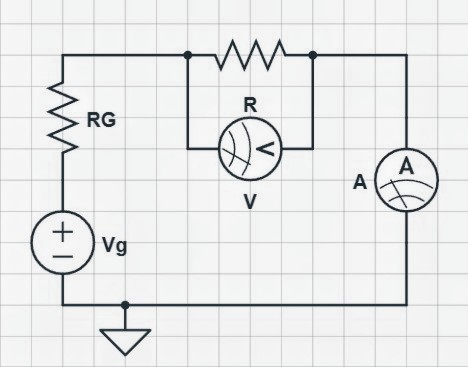
\includegraphics[width=0.5\textwidth]{grafici/config_1.jpg}
\captionof{figure}{configurazione 1 ideale}
\label{fig:1}
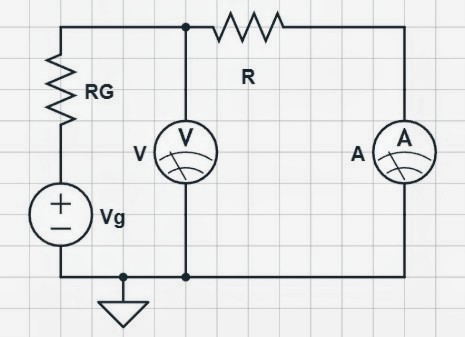
\includegraphics[width=0.5\textwidth]{grafici/config_2.jpg}
\captionof{figure}{configurazione 2 ideale}
\label{fig:2}
\end{center}

Per entrambe le configurazioni abbiamo raccolto almeno dieci misure della coppia corrente-tensione per due diversi resistori, uno con resistenza piccola ($10\si{\ohm}$) e uno con resistenza grande ($1\si{\mega\ohm}$).
Nell'utilizzare il carico resistivo più basso è stato possibile variare la tensione soltanto in un range ristretto di valori,
al fine di non raggiungere valori elevati di V così da evitare il passaggio di correnti troppo intense attraverso l'alimentatore o il multimetro da banco.
Abbiamo poi proceduto a determinare la resistenza interna dei multimetri, in modo tale da poterla confrontare con le resistenze inserite all'interno del circuito.
Sia amperometro che voltmetro nel caso reale si comportano infatti come delle resistenze, identificate come \( \mathit{R_a} \) e \( \mathit{R_v} \),
seppur idealmente gli strumenti di misura non dovrebbero influire sulle misure di corrente e tensione.
Lo schema reale, il quale tiene conto della presenza dei multimetri all'interno del circuito, è mostrato in figura \ref{fig:3} e \ref{fig:4}.
\begin{center}
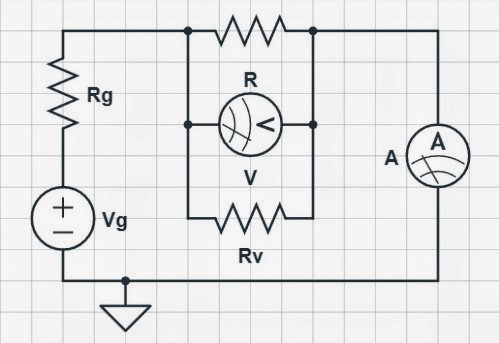
\includegraphics[width=0.5\textwidth]{grafici/conf_1_bias.jpg}
\captionof{figure}{configurazione 1 reale}
\label{fig:3}
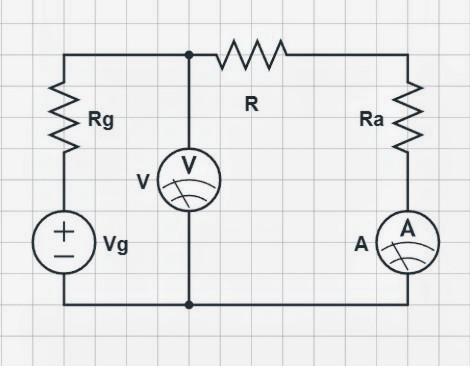
\includegraphics[width=0.5\textwidth]{grafici/conf_2_bias.jpg}
\captionof{figure}{configurazione 2 reale}
\label{fig:4}
\end{center}
A partire dall'analisi circuitale della configurazione reale abbiamo quindi ricavato la relazione necessaria a determinare le resistenze interne \( \mathit{R_a} \) e \( \mathit{R_v} \).
Definita \( \mathit{I} \) la corrente che circola all'interno del circuito, \( \mathit{V} \) la differenza di potenziale applicata ai suoi capi, e \( \mathit{R} \) la resistenza propria del resistore
si ha:
\begin{align}
	 & R_a = \frac {V}{I} - R \quad \text{e} \quad R_v = \frac {I}{V} - \frac{1}{R}\quad \label{eq:1}
\end{align}
Per determinare \( \mathit{R_v} \) è stata utilizzata la configurazione 1,
applicando la legge di Ohm al tratto di circuito contenente le resistenze \( \mathit{R} \) e \( \mathit{R_v} \), tra loro in parallelo.
Al contrario, per ricavare \( \mathit{R_a} \), le misurazioni sono state effettuate utilizzando la configurazione 2,
sfruttando sempre la legge di Ohm, ma considerando la resistenza equivalente alla serie delle resistenze \( \mathit{R} \) e \( \mathit{R_a} \).
In entrambi i casi abbiamo raccolto le misure della coppia \( \mathit{I-V} \) per 5 valori distinti di \( \mathit{R} \), impostata dalla cassetta di resistenze.
Confrontando ora \(R\) con le resistenze interne degli strumenti di misura è stato possibile valutare quale configurazione garantisse un bias minore sulle misure.
Per \(R = 10\si{\ohm}\) bassa rispetto alla resistenza del voltmetro si ottengono risultati più accurati scegliendo la configurazione \ref{fig:1}, in quanto la configurazione \ref{fig:2}
fornirebbe misure di \( V \) non corrispondenti alla differenza di potenziale ai capi della resistenza, ma anzi alla serie tra \(R\) e \(R_a\).
Al contrario per \(R=1\si{\mega\ohm}\) alta rispetto alla resistenza dell'amperometro, è preferibile la configurazione \ref{fig:2}.
Infatti se si utilizzasse la configurazione \ref{fig:1} l'amperometro misurerebbe una corrente che non corrisponde a quella che scorre attraverso la resistenza, poichè essa andrebbe a dividersi tra il tratto di circuito contenente \(R_v\) e quello contenente \(R\).
\subsection{Dati}
Riportiamo nella tabelle sottostanti le coppie di valori \(I-V\) misurati con entrambe le configurazioni, dapprima impostando una resistenza di $1\si{\mega\ohm}$ e poi una da $10\si{\ohm}$.
L'errore sulla tensione è stato stimato utilizzando la sensibilità del voltmetro: \( \si{\delta_{V}=0.01 V} \). Per le misure con \(R=1\si{\mega\ohm}\) per determinare l'incertezza relativa alle misure di corrente abbiamo osservato il valore di \(I\) restituito dall'amperometro nella situazione di circuito aperto, definendo quindi \( \si{\delta_{I}=0.003 {\micro\ampere}} \). Per le misure con \(R=10\si{\ohm}\) abbiamo invece valutato la fluttuazione delle misure di corrente lette dall'amperometro, dal momento che essere risultavano maggiori di $0.003 \si{\micro\ampere}$.
\begin{center}
\begin{tabular}{|c|c|c|c|}
\hline
$I_1$ $\times 10^{-8}[A]$ & $V_1$ $\times 10^{-2}[V]$ & $I_2$ $\times 10^{-8}[A]$ & $V_2$ $\times 10^{-2}[V]$ \\
\hline
$6 \pm 3$ & $1 \pm 1$ & $3 \pm 3$ & $1 \pm 1$ \\
$114 \pm 3$ & $101 \pm 1$ & $104 \pm 3$ & $102 \pm 1$ \\
$222 \pm 3$ & $200 \pm 1$ & $202 \pm 3$ & $200 \pm 1$ \\
$331 \pm 3$ & $300 \pm 1$ & $303 \pm 3$ & $301 \pm 1$ \\
$443 \pm 3$ & $403 \pm 1$ & $403 \pm 3$ & $400 \pm 1$ \\
$551 \pm 3$ & $501 \pm 1$ & $502 \pm 3$ & $500 \pm 1$ \\
$675 \pm 3$ & $616 \pm 1$ & $603 \pm 3$ & $601 \pm 1$ \\
$775 \pm 3$ & $702 \pm 1$ & $707 \pm 3$ & $705 \pm 1$ \\
$886 \pm 3$ & $802 \pm 1$ & $803 \pm 3$ & $800 \pm 1$ \\
$997 \pm 3$ & $902 \pm 1$ & $903 \pm 3$ & $900 \pm 1$ \\
$1104 \pm 3$ & $1001 \pm 1$ & $1007 \pm 3$ & $1004 \pm 1$ \\
$1216 \pm 3$ & $1103 \pm 1$ & $1108 \pm 3$ & $1104 \pm 1$ \\
$1322 \pm 3$ & $1200 \pm 1$ & $1202 \pm 3$ & $1199 \pm 1$ \\
$1434 \pm 3$ & $1301 \pm 1$ & $1303 \pm 3$ & $1300 \pm 1$ \\
$1548 \pm 3$ & $1404 \pm 1$ & $1404 \pm 3$ & $1400 \pm 1$ \\
$1653 \pm 3$ & $1500 \pm 1$ & $1504 \pm 3$ & $1501 \pm 1$ \\
$1762 \pm 3$ & $1600 \pm 1$ & $1605 \pm 3$ & $1602 \pm 1$ \\
$1873 \pm 3$ & $1700 \pm 1$ & $1704 \pm 3$ & $1701 \pm 1$ \\
$1984 \pm 3$ & $1801 \pm 1$ & $1804 \pm 3$ & $1800 \pm 1$ \\
$2093 \pm 3$ & $1900 \pm 1$ & $1906 \pm 3$ & $1903 \pm 1$ \\
$2204 \pm 3$ & $2001 \pm 1$ & $2003 \pm 3$ & $2000 \pm 1$ \\
\hline
\end{tabular}
\captionof{table}{resistenza $1\si{\mega\ohm}$}
\vspace{0.3cm}
\begin{tabular}{|c|c|c|c|}
\hline
$I_1$ $\times 10^{-5}$ [A]& $V_1$ $\times 10^{-2}$ [V]& $I_2$ $\times 10^{-6}$ [A]& $V_2$ $\times 10^{-2}$ [V]\\
\hline
$12.039 \pm 0.002$ & $0 \pm 1$ & $168.30 \pm 0.02$ & $2 \pm 1$ \\
$5920 \pm 1$ & $53 \pm 1$ & $45591.00 \pm 0.01$ & $50 \pm 1$ \\
$11229 \pm 1$ & $100 \pm 1$ & $95510 \pm 10$ & $101 \pm 1$ \\
$16817 \pm 1$ & $151 \pm 1$ & $145610 \pm 20$ & $154 \pm 1$ \\
$22394 \pm 1$ & $201 \pm 1$ & $190020 \pm 10$ & $200 \pm 1$ \\
$27907 \pm 1$ & $250 \pm 1$ & $239410 \pm 10$ & $253 \pm 1$ \\
$33541 \pm 3$ & $301 \pm 1$ & $284450 \pm 10$ & $300 \pm 1$ \\
$39240 \pm 5$ & $353 \pm 1$ & $334040 \pm 10$ & $354 \pm 1$ \\
$44400 \pm 4$ & $400 \pm 1$ & $378750 \pm 100$ & $401 \pm 1$ \\
$49920 \pm 10$ & $450 \pm 1$ & $424040 \pm 50$ & $450 \pm 1$ \\
0 & $0 \pm 1$ & $473200 \pm 100$ & $504 \pm 1$ \\
\hline
\end{tabular}
\captionof{table}{resistenza $10 \si{\ohm}$}
\end{center}

Nelle tabelle seguenti sono invece visibili i valori di tensione, corrente e resistenza utilizzati per ricavare le resistenze interne dei multimetri.
L'incertezza sui valori di \(I\) e di \(V\) è stata ricavata come nel caso precedente, mentre per \(R\) abbiamo considerato l'errore relativo riportato sulla cassetta di resistenze, pari all'1\%.

\begin{center}
\begin{tabular}{|l|c c c c c|}
\hline
I $\times 10^{-6}[A]$ & $47052 \pm 1$ & $23785 \pm 1$ & $15966 \pm 1$ & $11925 \pm 1$ & $9586 \pm 1$ \\
\hline
V $\times 10^{-3}[V]$ & $4804 \pm 1$ & $4804 \pm 1$ & $4804 \pm 1$ & $4804 \pm 1$ & $4804 \pm 1$ \\
\hline
R [$\si{\ohm}]$ & $100 \pm 1$ & $200 \pm 2$ & $300 \pm 3$ & $400 \pm 4$ & $500 \pm 5$ \\
\hline
\end{tabular}
\captionof{table}{caratterizzazione amperometro}
\vspace{10mm}
\begin{tabular}{|l|c c c c c|}
\hline
I $\times 10^{-8}[A]$ & $207 \pm 1$ & $166 \pm 1$ & $126 \pm 1$ & $142 \pm 1$ & $530 \pm 1$ \\
\hline
V $\times 10^{-3}[V]$ & $4835 \pm 1$ & $4835 \pm 1$ & $4835 \pm 1$ & $4835 \pm 1$ & $4835 \pm 1$ \\
\hline
R $\times 10^{4}[$\si{\ohm}] & $300 \pm 3$ & $400 \pm 4$ & $600 \pm 6$ & $500 \pm 5$ & $100 \pm 1$ \\
\hline
\end{tabular}
\captionof{table}{caratterizzazione voltometro}
\end{center}

\subsection{Analisi dati}
Considerando le misure effettuate per ciascuna configurazione e per ciascuna resistenza, abbiamo fittato i dati con una relazione lineare, come previsto dalla Legge di Ohm \( V = RI \) e come mostrato dai seguenti grafici.

\begin{center}
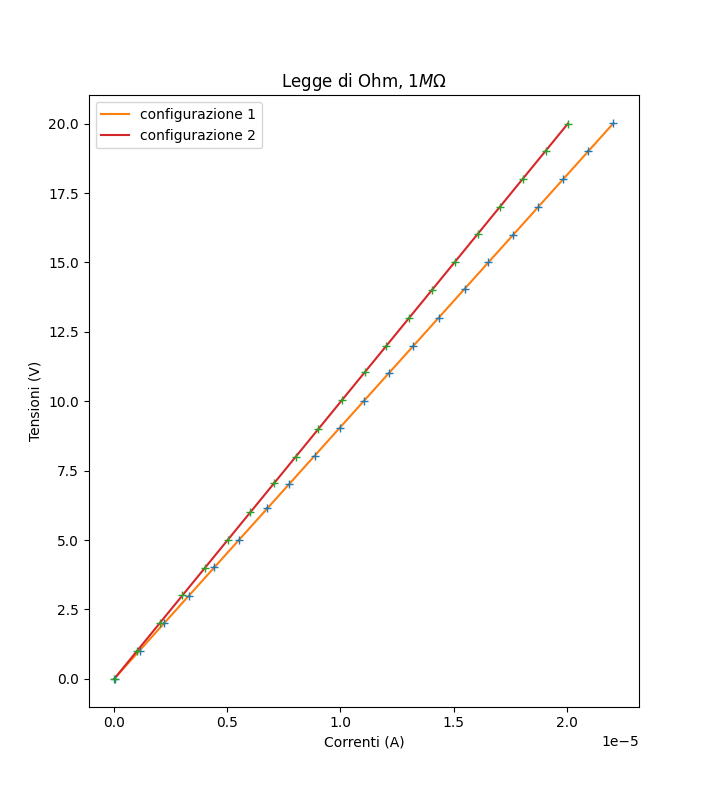
\includegraphics[width=0.7\textwidth]{grafici/ohm_resistenza_alta.png}
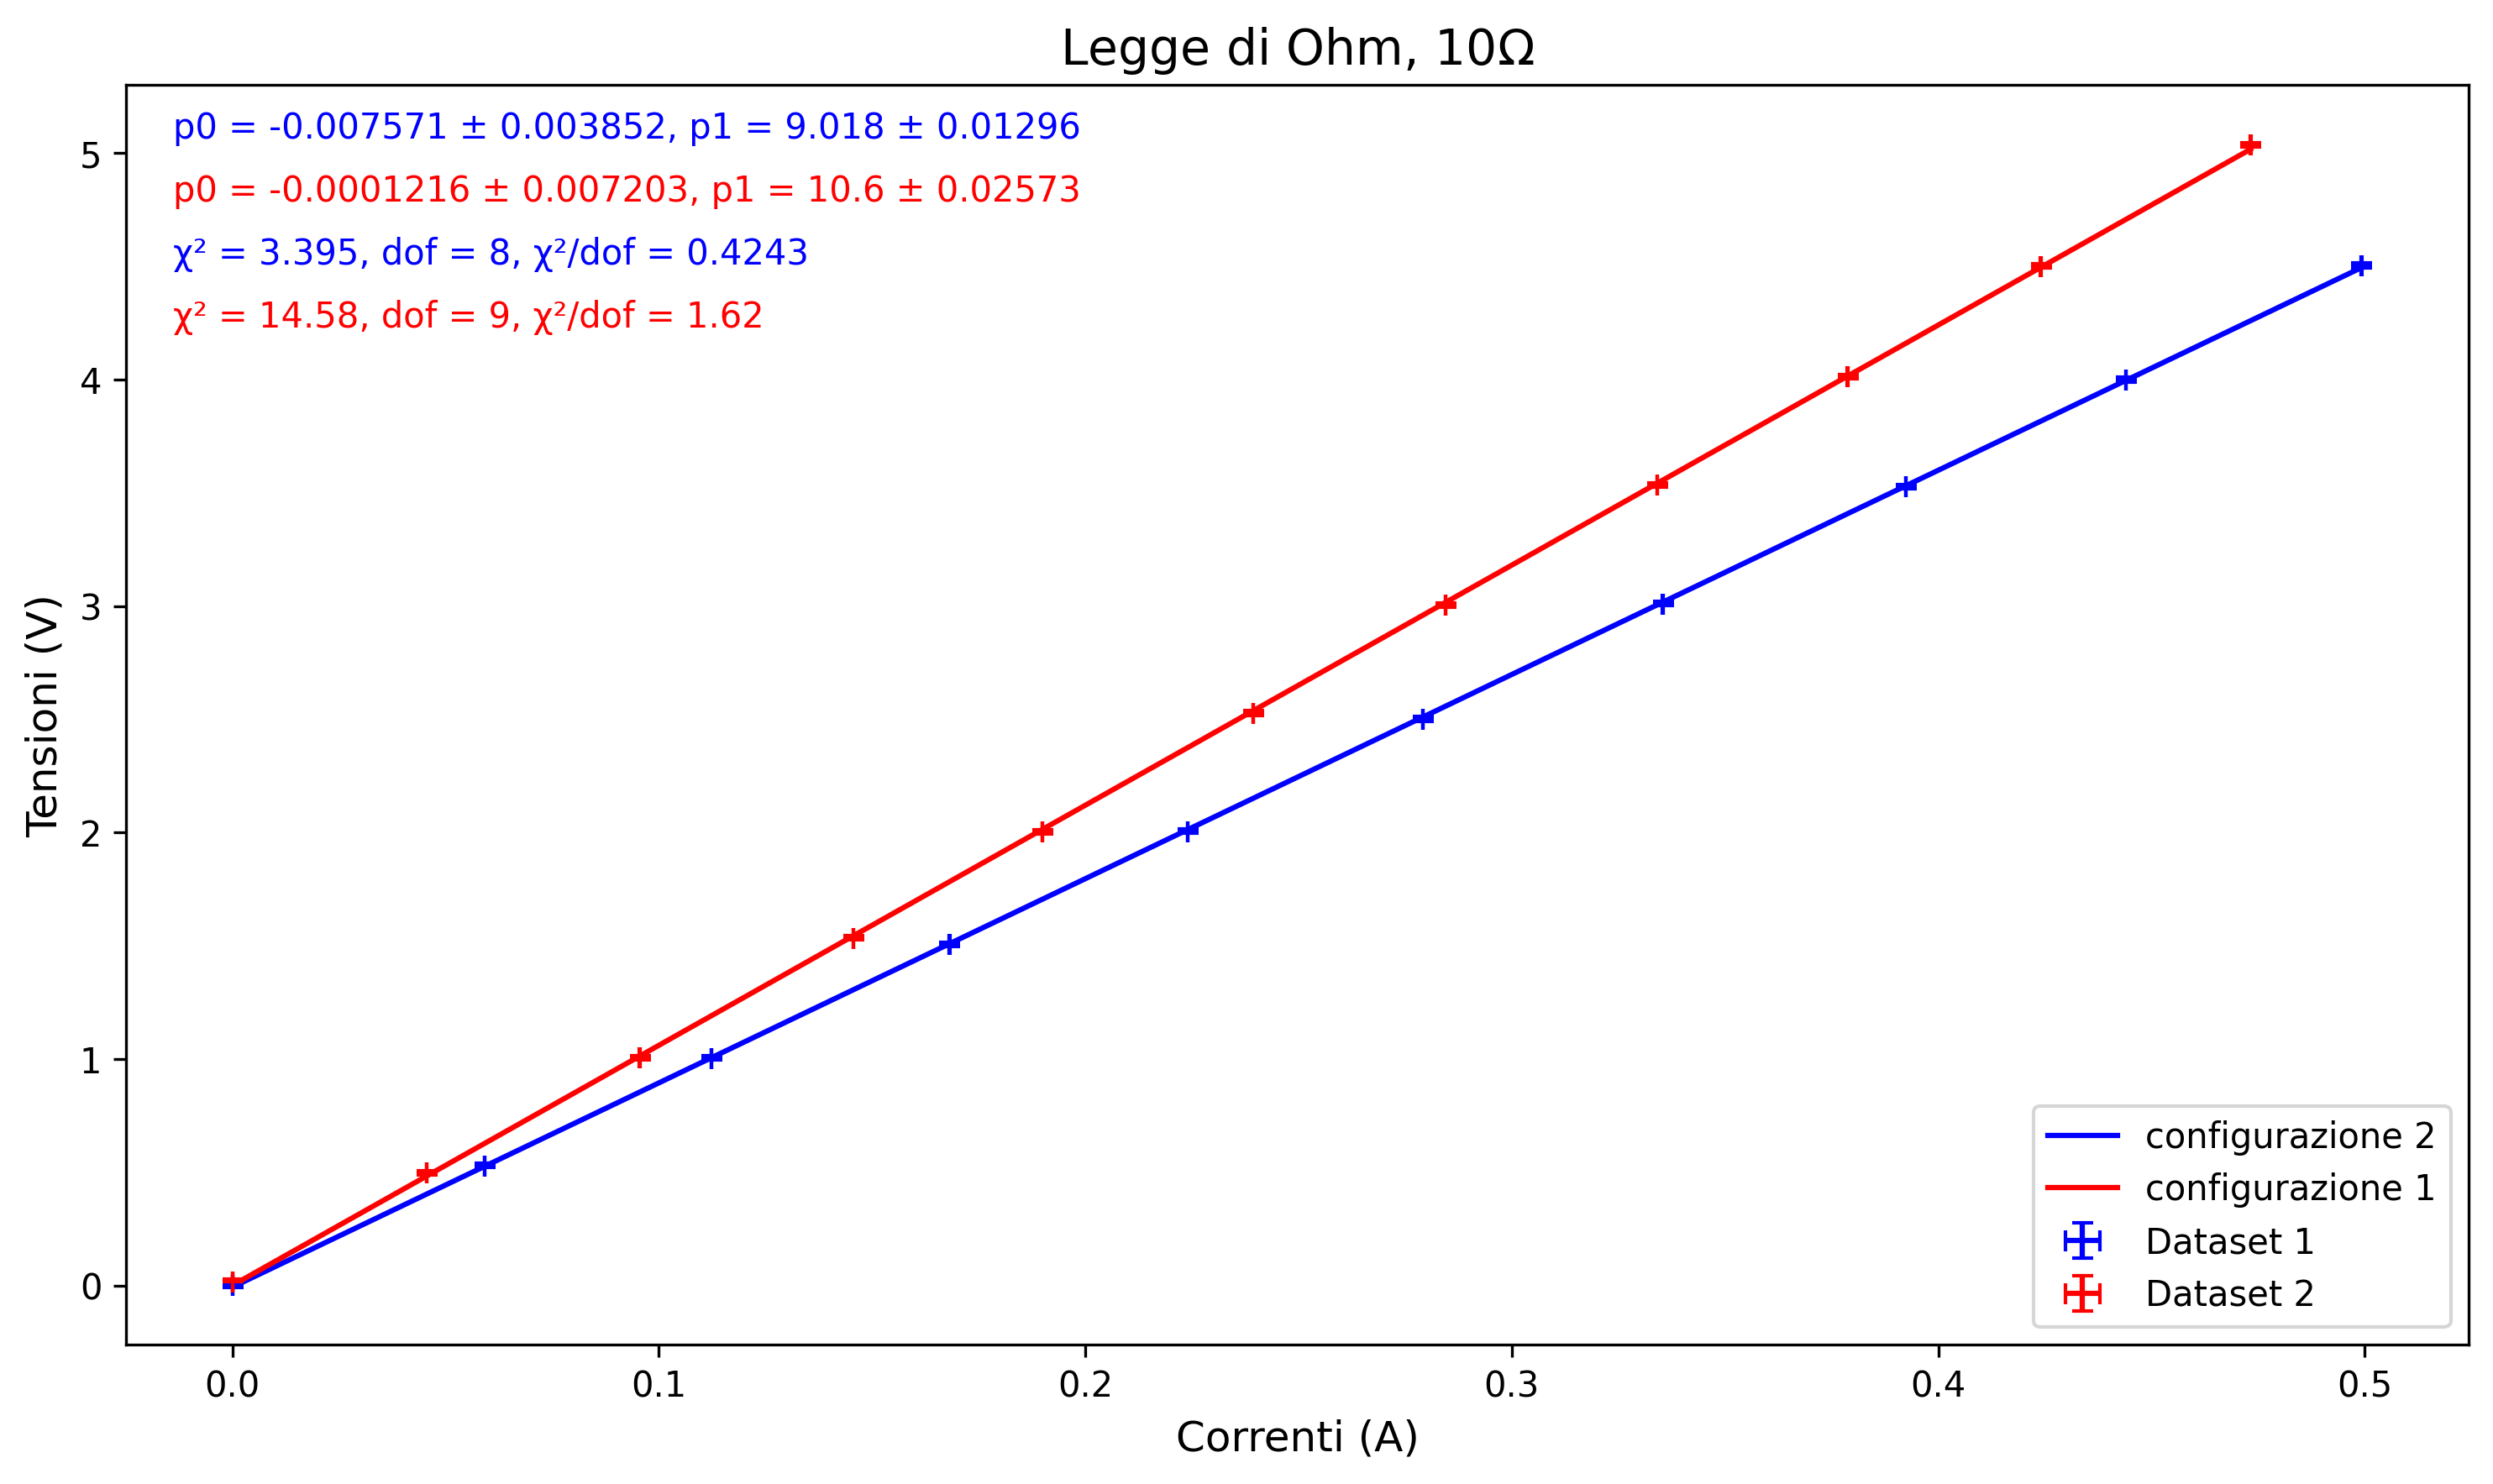
\includegraphics[width=0.7\textwidth]{grafici/ohm_resistenza_bassa.png}
\end{center}

I parametri che descrivono la relazione tensione-corrente ricavati mediante interpolazione lineare sono riportati in seguito, affiancati dal proprio errore. \( \mathit{m} \) e \( \mathit{a} \) indicano rispettivamente il coefficiente angolare della retta e la sua intercetta. Dal confronto con la Legge di Ohm imponiamo poi \( m = R \) e \( \delta_{m} = \delta_{R} \).

\begin{center}
\begin{tabular}{|c|c|c|c|}
\hline
$m_1$ & $a_1$ & $m_2$ & $a_2$ \\
\hline
$908470 \pm 494$ & $0.014 \pm 0.006$ & $999234 \pm 179$ & $0.020 \pm 0.002$\\
\hline
\end{tabular}
\captionof{table}{$R_{\text{atteso}}=1 \si{\mega\ohm}$}
\end{center}
\begin{center}
\begin{tabular}{|c|c|c|c|}
\hline
$m_1$ & $a_1$ & $m_2$ & $a_2$ \\
\hline
$10.60 \pm 0.03$ & $-0.0001 \pm 0.0072$ & $9.02 \pm 0.01$ & $-0.008 \pm 0.003$\\
\hline
\end{tabular}
\captionof{table}{$R_{\text{atteso}}=10 \si{\ohm}$}
\end{center}

Abbiamo quindi effettuato il test di compatibilità tra le misure di resistenza ricavate utilizzando la prima configurazione (\(R_1\)) e le misure determinate mediante la seconda configurazione (\(R_2\)). Gli esiti, visibili in seguito, mostrano la probabilità entro \(t\) sigma con \( t = \frac {R_1 - R_2}{\sqrt{\delta_{R_1}^2+\delta_{R_2}^2}} \).

\begin{center}
\begin{tabular}{|l|c|}
\hline
probabilità entro t sigma & 1 \\
\hline
\end{tabular}
\captionof{table}{$R_{\text{atteso}}=1 \si{\mega\ohm}$}
\end{center}

\begin{center}
\begin{tabular}{|l|c|}
\hline
probabilità entro t sigma & 0.99 \\
\hline
\end{tabular}
\captionof{table}{$R_{\text{atteso}}=10 \si{\ohm}$}
\end{center}

Come si può osservare i risultati delle due configurazione non appaiono tra loro compatibili: tale incompatibilità trova spiegazione nella non idealità dei multimetri. Nel caso ideale, in cui \(R_a = 0\) e \(R_v \approx \infty\), le due configurazioni dovrebbero fornire gli stessi risultati, ma in quello reale i parametri ricavati mediante interpolazione sono affetti da bias, dipendente dai valori di \(R_a\) e \(R_v\). 
Abbiamo quindi ricavato i valori \(R_a\) e \(R_v\), riportati nella tabella sottostante, come spiegato in precedenza. Utilizzando le relazioni (\ref{eq:1}) abbiamo calcolato 5 valori di \(R_a\) e \(R_v\), dei quali abbiamo considerato poi media e deviazione standard sulla media, stimando così la resistenza interna dei multimetri e la sua incertezza. 

\begin{center}
\begin{tabular}{|c|c|}
\hline
$R_a$ & $R_v$ \\
\hline
$1.8 \pm 0.7$ & $10596156 \pm 113146$ \\
\hline
\end{tabular}
\captionof{table}{resistenze interne multimetri}
\end{center}

Al fine di quantificare il bias abbiamo poi osservato, a partire dall'analisi circuitale dei circuiti riportati in figura 3 e 4, come la relazione $R=\frac{V}{I}$ sia in realtà esatta soltanto considerando come $R$ la resistenza equivalente. In particolar modo per la configurazione 1 e per la configurazione 2 otteniamo rispettivamente:
\begin{align*}
	R_{1,\text{eq}}=\frac{RR_v}{R+R_v} \quad \text{e} \quad R_{2,\text{eq}}=R+R_a
\end{align*}
Ne consegue che le misure di $R$ sono affette da bias pari a:
\begin{align*}
	 & \text{bias}_1= R-\left(\frac{RR_v}{R+R_v}\right)  \quad \text{e} \quad \text{bias}_2=R-(R+R_a)
\end{align*}
Tenendo conto del ragionamento precedente, per calcolare $\text{bias}_1$ abbiamo considerato $R = 10\si{\ohm}$ (configurazione 1 migliore per resistenza piccola), mentre per $\text{bias}_2$ abbiamo sostituito il valore di $R=1\si{\mega\ohm}$ (configurazione 2 migliore per resistenza grande).
In seguito riportiamo i valori di tali bias.

\begin{center}
\begin{tabular}{|c|c|}
\hline
$\text{bias}_1$ & $\text{bias}_2$ \\
\hline
$9.44\times 10^{-6}$ & $1.79$ \\
\hline
\end{tabular}
\captionof{table}{bias di misura}
\end{center}

Possiamo quindi osservare $\text{bias}_1 < \delta_{R_1} = 179$ e $\text{bias}_2 < \delta_{R_2} = 0.03$; essendo minori dell'incertezza di misura possono essere trascurati.
Dopodichè abbiamo valutato la compatibilità dei valori delle resistenze inserite nel circuito con i valori di $R$ ricavati con entrambe le configurazioni. Per fare ciò è stato utilizzato il t-test con $t = \frac {R - R_{\text{nota}}}{\sqrt{\delta_{R}^2+\delta_{R_{\text{nota}}}^2}}$, i cui esiti sono raccolti in tabella.

\begin{center}
\begin{tabular}{|l|c|c|}
\hline
probabilità entro t sigma & t1=1 & t2=0.06 \\
\hline
\end{tabular}
\captionof{table}{$R_{\text{atteso}}=1 \si{\mega\ohm}$}
\end{center}

\begin{center}
\begin{tabular}{|l|c|c|}
\hline
probabilità entro t sigma & t1=1 & t2=1 \\
\hline
\end{tabular}
\captionof{table}{$R_{\text{atteso}}=10 \si{\ohm}$}
\end{center}

Infine i parametri di fit e le misure realizzate sono stati utilizzati per effettuare il test del chi quadro, in modo da poter verificare la validità della Legge di Ohm. I risultati sono visibili all'interno del grafico.


\subsection{Conclusione}
Sulla base degli esiti positivi del test del chi quadro possiamo considerare come verificata la Legge in Ohm, in quanto la relazione corrente-tensione risulta esprimibile mediante una retta del tipo \(y= mx\).
Guardando a quanto ricavato per \(R=1\si{\mega\ohm}\), il t-test ha dimostrato la compatibilità dei valori di resistenza noti con quelli ricavati sperimentalmente utilizzando la configurazione 2. Al contrario, come ci aspettavamo, il test di compatibilità ha avuto esito negativo considerando la configurazione 1. Invece per \(R = 10\si{\ohm}\) non si ha accordo con quanto ricavato sperimentalmente, nè con la configurazione 1 nè con la configurazione 2. Attribuiamo tale risultato al fatto che la tensione imposta dalla cassetta di resistenze non corrispondesse a quanto ivi indicato.


%%%%%%%%%%%%%%%%%%%%%%%%%%%%%%%%%%%%%%%%%%%%%%%%%%%%%%%%%%%%%%%%%%%%%%%%%%%%%%%%%%%%%%%%%%%%%%%%%%
\section{Partitore resistivo}
\subsection{Obiettivo}
Realizzare un circuito contenente tre diverse resistenze: \emph{$R_1, R_2, R_{\text{load}}$} strutturato come in figura \ref{fig:partitore}.
Il circuito deve essere dimensionato in modo tale che la caduta di potenziale ai capi della resistenza di carico \( \mathit{R_{load}} \) non dipenda dal valore di resistenza del carico.
Inoltre \( \mathit{R_1} \) e \( \mathit{R_2} \) devono essere scelte in modo che \( \mathit{V_{\text{in}}} \) sia circa \( \mathit{0.5 V_{\text{out}}} \).
\( \mathit{V_{\text{in}}} \) rappresenta la caduta di potenziale dovuta a $R_1 + R_2$, mentre \( \mathit{V_{\text{out}}} \) indica la caduta di potenziale dovuta solo a $R_2$, nel caso in cui $R_{\text{load}}$ sia appunto ininfluente.
\begin{center}
	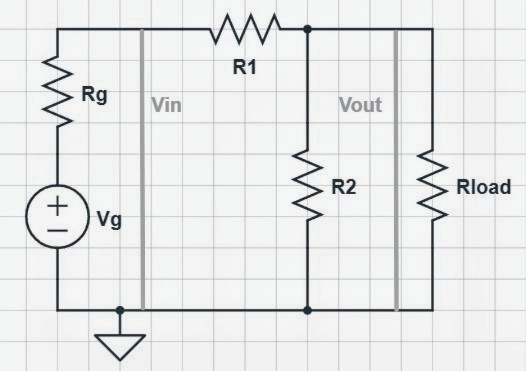
\includegraphics[width=0.5\textwidth]{grafici/partitore.jpg}
	\captionof{figure}{Partitore resistivo}
	\label{fig:partitore}
\end{center}
\subsection{Metodo}
Abbiamo realizzato il partitore resistivo utilizzando la breadbord, nella quale abbiamo inserito le resistenze $R_1$ e $R_2$,
e collegandola al generatore e alla cassetta di resistenze, scelta per rappresentare $R_{\text{load}}$, così da poterne variare agevolmente i valori.
Al fine di rendere il valore della differenza di potenziale $V_{\text{out}}$ costante, cioè indipendente da $R_{\text{load}}$,
$R_{\text{load}}$ deve assumere valori molto elevati, così che la corrente scorra principalmente nel tratto di circuito non contenente $R_{\text{load}}$
e quindi non si abbia caduta di potenziale ai suoi capi.
Di fatto la corrente sceglie il percorso contenente $R_1$ e $R_2$.
Per avere $V_{\text{in}} \approx 0.5V_{\text{out}}$ le due cadute di tensione ai capi di $R_1$ e $R_2$ devono essere identiche, ossia, essendo attraversate dalla stessa corrente, $R_1=R_2$.
Utilizzando le resistenze a disposizione abbiamo potuto garantire soltanto $R_1\approx R_2$, e non una esatta corrispondenza, infatti $R_1=21.67 \si{\ohm}$ e $R_2=21.65 \si{\ohm}$.
Dopo aver realizzato il partitore resistivo sulla breadboard, per verificare che esso rispetti le caratteristiche richieste, è stato necessario inserirvi il voltmetro,
così da poter misurare i valori di $V_{\text{in}}$ e $V_{\text{out}}$. Per misurare $V_{\text{in}}$ il voltmetro è stato inserito in parallelo con l'alternatore,
mentre per la misura di $V_{\text{out}}$ lo abbiamo collegato in parallelo con $R_{\text{load}}$ (e quindi anche con la resistenza equivalente a $R_1$ e $R_2$).
Abbiamo quindi effettuato 5 misure di $V_{\text{in}}$ e $V_{\text{out}}$ al variare di $R_{\text{load}}$ tra 1 \si{\mega\ohm} e 5 \si{\mega\ohm},  mantenendo costante la tensione erogata dal generatore.
\subsection{Dati}
Nella tabella sottostante sono riportati i valori di $V_{\text{in}}$, $V_{\text{out}}$ e $R_{\text{load}}$ con i rispettivi errori.
Le incertezze di $V_{\text{in}}$ e $V_{\text{out}}$ sono state stimate utilizzando la sensibilità del voltmetro, quindi $\delta_{V_{\text{in}}}=\delta_{V_{\text{out}}}=0.001 V$;
mentre per determinare $\delta_{R_{\text{load}}}$ abbiamo preso in considerazione l'errore relativo dell'1\% indicato sulla cassetta di resistenze.

\begin{center}
\begin{tabular}{|l|c c c c c|}
\hline
\(V_{in}\) $[V]$ & $2.164 \pm 0.001$ & $2.164 \pm 0.001$ & $2.164 \pm 0.001$ & $2.164 \pm 0.001$ & $2.164 \pm 0.001$ \\
\hline
\(V_{out}\) $[V]$ & $1.069 \pm 0.001$ & $1.075 \pm 0.001$ & $1.077 \pm 0.001$ & $1.078 \pm 0.001$ & $1.078 \pm 0.001$ \\
\hline
\(R\) $\times 10^6[\si{\ohm}]$ & $1 \pm 0.01$ & $2 \pm 0.02$ & $3 \pm 0.03$ & $4 \pm 0.04$ & $5 \pm 0.05$ \\
\hline
\end{tabular}
\captionof{table}{partitore resistivo}
\end{center}

\subsection{Analisi dati}
Il grafico sotto riportato rappresenta le coppie di valori $V_{\text{out}}$-$R_{\text{load}}$ con i relativi errori.

\begin{center}
    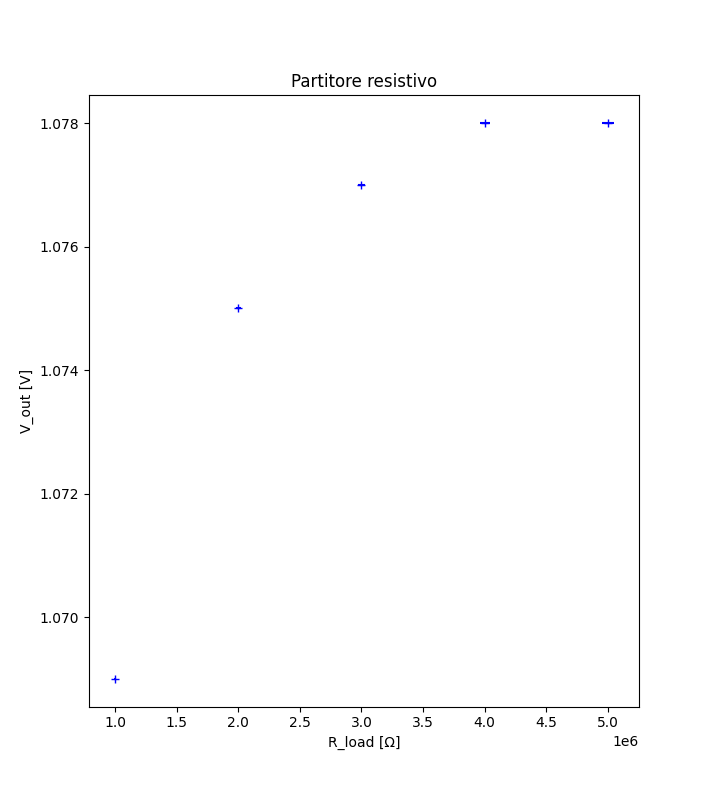
\includegraphics[width=0.5\textwidth]{grafici/partitore_resistivo.png}
\end{center}
\subsection{Conclusione}
Come si può osservare dal grafico il valore della resistenza di carico non è completamente ininfluente su $V_{\text{out}}$.
Al variare di $R_{\text{load}}$ si hanno infatti fluttuazioni di $V_{\text{out}}$; indice del fatto che, seppur $R_{\text{load}}$ sia molto elevata, essa ha un valore finito e quindi
parte della corrente continua a fluire all'interno del componente resistivo. A conferma di ciò possiamo osservare come si raggiungano valori di $V_{\text{out}}$ più alti all'aumentare di $R_{\text{load}}$.
Inoltre, come atteso, per $R_1 \approx R_2$ si ha $V_{\text{in}} \approx 0.5V_{\text{out}}$.

%%%%%%%%%%%%%%%%%%%%%%%%%%%%%%%%%%%%%%%%%%%%%%%%%%%%%%%%%%%%%%%%%%%%%%%%%%%%%%%%%%%%%%%%%%
\section{Caratteristica tensione-corrente di un diodo}
\subsection{Obiettivo}
Misurare tensione e corrente ai capi di un diodo e verificare che le informazioni raccolte rispettino quanto previsto dalla legge di Shockley: $I = I_0 \left( e^{\frac{qV}{gkT}} - 1 \right)$.
Dove $I$ è la corrente che attraversa il diodo mentre $V$ è la tensione applicata. $I_0$ indica invece la corrente di saturazione inversa, $g$ è una costante dipendente dal diodo,
$k$ è la costante di Boltzmann ($1.38 \times 10^{-23} \, \text{J/K}$), $T$ è la temperatura in Kelvin, e $q$ è la carica dell'elettrone ($1.60 \times 10^{-19}$ C).
Utilizzare poi i dati per stimare la costante del diodo $g$ e la corrente di saturazione inversa $I_0$.
\subsection{Metodo}
Abbiamo innanzitutto realizzato il circuito, ripetendo la proceduta utilizzata per la verifica della Legge di Ohm, inserendo all'interno della breadboard il diodo e scollegandola dalla cassetta di resistenze.
Per compiere le misurazioni di corrente e tensione sono state utilizzate per il collegamento dei multimetri sia la configurazione \ref{fig:1} che la configurazione \ref{fig:2},
per ciascuna delle quali abbiamo raccolto 21 misure della coppia \( I-V \). A partire dai valori di tensione e corrente abbiamo poi ricavato la resistenza equivalente,
dipendente dalla tensione tramite la relazione \( R_{eq} = \frac {V}{I} \), di conseguenza non costante; il diodo rappresenta infatti un componente non Ohmico.
Dal confronto di $R_{\text{eq}}$ con le resistenze interne degli strumenti di misura è stato possibile supporre quale configurazione garantisse misurazioni più accurate.
Abbiamo proceduto con un ragionamento analogo a quello effettuato in precendenza per il calcolo del valore della resistenza, ricavando quindi che per $R_{\text{eq}}$ basse rispetto alla resistenza del voltometro è preferibile la configurazione \ref{fig:1}, mentre, per $R_{\text{eq}}$ alte rispetto alla resistenza dell'amperometro, la configurazione \ref{fig:2} rappresenta la scelta migliore.
\subsection{Dati}
Riportiamo nelle tabelle qui di seguito i valori di \(V\) e \(I\), affiancati dalla corrispettiva \(R_{\text{eq}}\), e relativi alle misure sul diodo per entrambe le configurazioni. L'errore su \(V\) e \(I\) è stato stimato considerando la fluttuazione dei valori mostrati dagli strumenti di misura.

\begin{center}
\begin{tabular}{|c|c|c|}
\hline
$I \times 10^{-3}[A]$ & $V \times 10^{-3}[V]$ & $R_{\text{eq}}$ [$\si{\ohm}$]\\
\hline
$0.00003 \pm 0.00001$ & $100 \pm 1$ & 3.33 \\
$0.00005 \pm 0.00001$ & $212 \pm 1$ & 4.24 \\
$0.0002 \pm 0.00002$ & $309 \pm 1$ & 1.54 \\
$0.00341 \pm 0.00001$ & $396 \pm 1$ & 0.116 \\
$0.0769 \pm 0.0001$ & $501 \pm 1$ & 0.00652 \\
$0.91 \pm 0.002$ & $600 \pm 1$ & 0.000659 \\
$10.5 \pm 0.4$ & $700 \pm 1$ & $6.67 \times 10^{-5}$ \\
$109 \pm 1$ & $796 \pm 1$ & $7.3 \times 10^{-6}$ \\
$490 \pm 1$ & $880 \pm 1$ & $1.8 \times 10^{-6}$ \\
$0.253 \pm 0.003$ & $559 \pm 1$ & 0.00221 \\
$2.764 \pm 0.002$ & $655 \pm 1$ & 0.000237 \\
$4.653 \pm 0.002$ & $675 \pm 1$ & 0.000145 \\
$32.9 \pm 0.1$ & $746 \pm 1$ & $2.27 \times 10^{-5}$ \\
$64 \pm 0.5$ & $773 \pm 1$ & $1.21 \times 10^{-5}$ \\
$253 \pm 1$ & $836 \pm 1$ & $3.3 \times 10^{-6}$ \\
$214 \pm 1$ & $823 \pm 1$ & $3.85 \times 10^{-6}$ \\
$1.14 \pm 0.01$ & $624 \pm 1$ & 0.000545 \\
$0.00459 \pm 0.00001$ & $421 \pm 1$ & 0.0917 \\
$1.661 \pm 0.001$ & $638 \pm 1$ & 0.000384 \\
$18.1 \pm 0.1$ & $724 \pm 1$ & $4 \times 10^{-5}$ \\
$55 \pm 1$ & $762 \pm 1$ & $1.38 \times 10^{-5}$ \\
\hline
\end{tabular}
\captionof{table}{configurazione 1}
\end{center}

\begin{center}
\begin{tabular}{|c|c|c|}
\hline
$I \times 10^{-6}[A]$ & $V \times 10^{-3}[V]$ & $R_{\text{eq}}$ [$\si{\ohm}$]\\
\hline
$0.02 \pm 0.01$ & $16 \pm 1$ & 0.78 \\
$0.02 \pm 0.01$ & $18 \pm 1$ & 0.857 \\
$0.03 \pm 0.01$ & $105 \pm 1$ & 3.5 \\
$0.03 \pm 0.01$ & $207 \pm 1$ & 6.68 \\
$0.05 \pm 0.01$ & $258 \pm 1$ & 5.16 \\
$0.12 \pm 0.01$ & $305 \pm 1$ & 2.54 \\
$0.65 \pm 0.01$ & $360 \pm 1$ & 0.554 \\
$2.37 \pm 0.02$ & $401 \pm 1$ & 0.169 \\
$3.88 \pm 0.02$ & $418 \pm 1$ & 0.108 \\
$9.64 \pm 0.02$ & $447 \pm 1$ & 0.0464 \\
$19.5 \pm 0.1$ & $473 \pm 1$ & 0.0243 \\
$49.3 \pm 0.1$ & $509 \pm 1$ & 0.0103 \\
$78 \pm 0.1$ & $529 \pm 1$ & 0.00678 \\
$120.2 \pm 0.2$ & $550 \pm 1$ & 0.00458 \\
$176.7 \pm 0.2$ & $570 \pm 1$ & 0.00323 \\
$359 \pm 1$ & $616 \pm 1$ & 0.00172 \\
$410 \pm 1$ & $626 \pm 1$ & 0.00153 \\
$550 \pm 2$ & $652 \pm 1$ & 0.00119 \\
$951 \pm 2$ & $713 \pm 1$ & 0.00075 \\
$1214 \pm 2$ & $749 \pm 1$ & 0.000617 \\
$1658 \pm 2$ & $805 \pm 1$ & 0.000486 \\
\hline
\end{tabular}
\captionof{table}{configurazione 2}
\end{center}

\subsection{Analisi dati}
Di seguito si riportano i grafici ottenuti dall'interpolazione esponenziale dei dati raccolti precedentemente. Per il grafico  $I$-$V$ ci aspettiamo un andamento esponenziale dato dalla legge di Shockley:  $I = I_0 \left( e^{\frac{qV}{gkT}} - 1 \right)$ già esposta in precedenza. I valori di $k$ e $q$ sono noti e costanti, per quanto riguarda la temperatura $T$ consideriamo la temperatura dell'ambiente  $T=300K$ e la ipotizziamo costante.

\begin{center}
    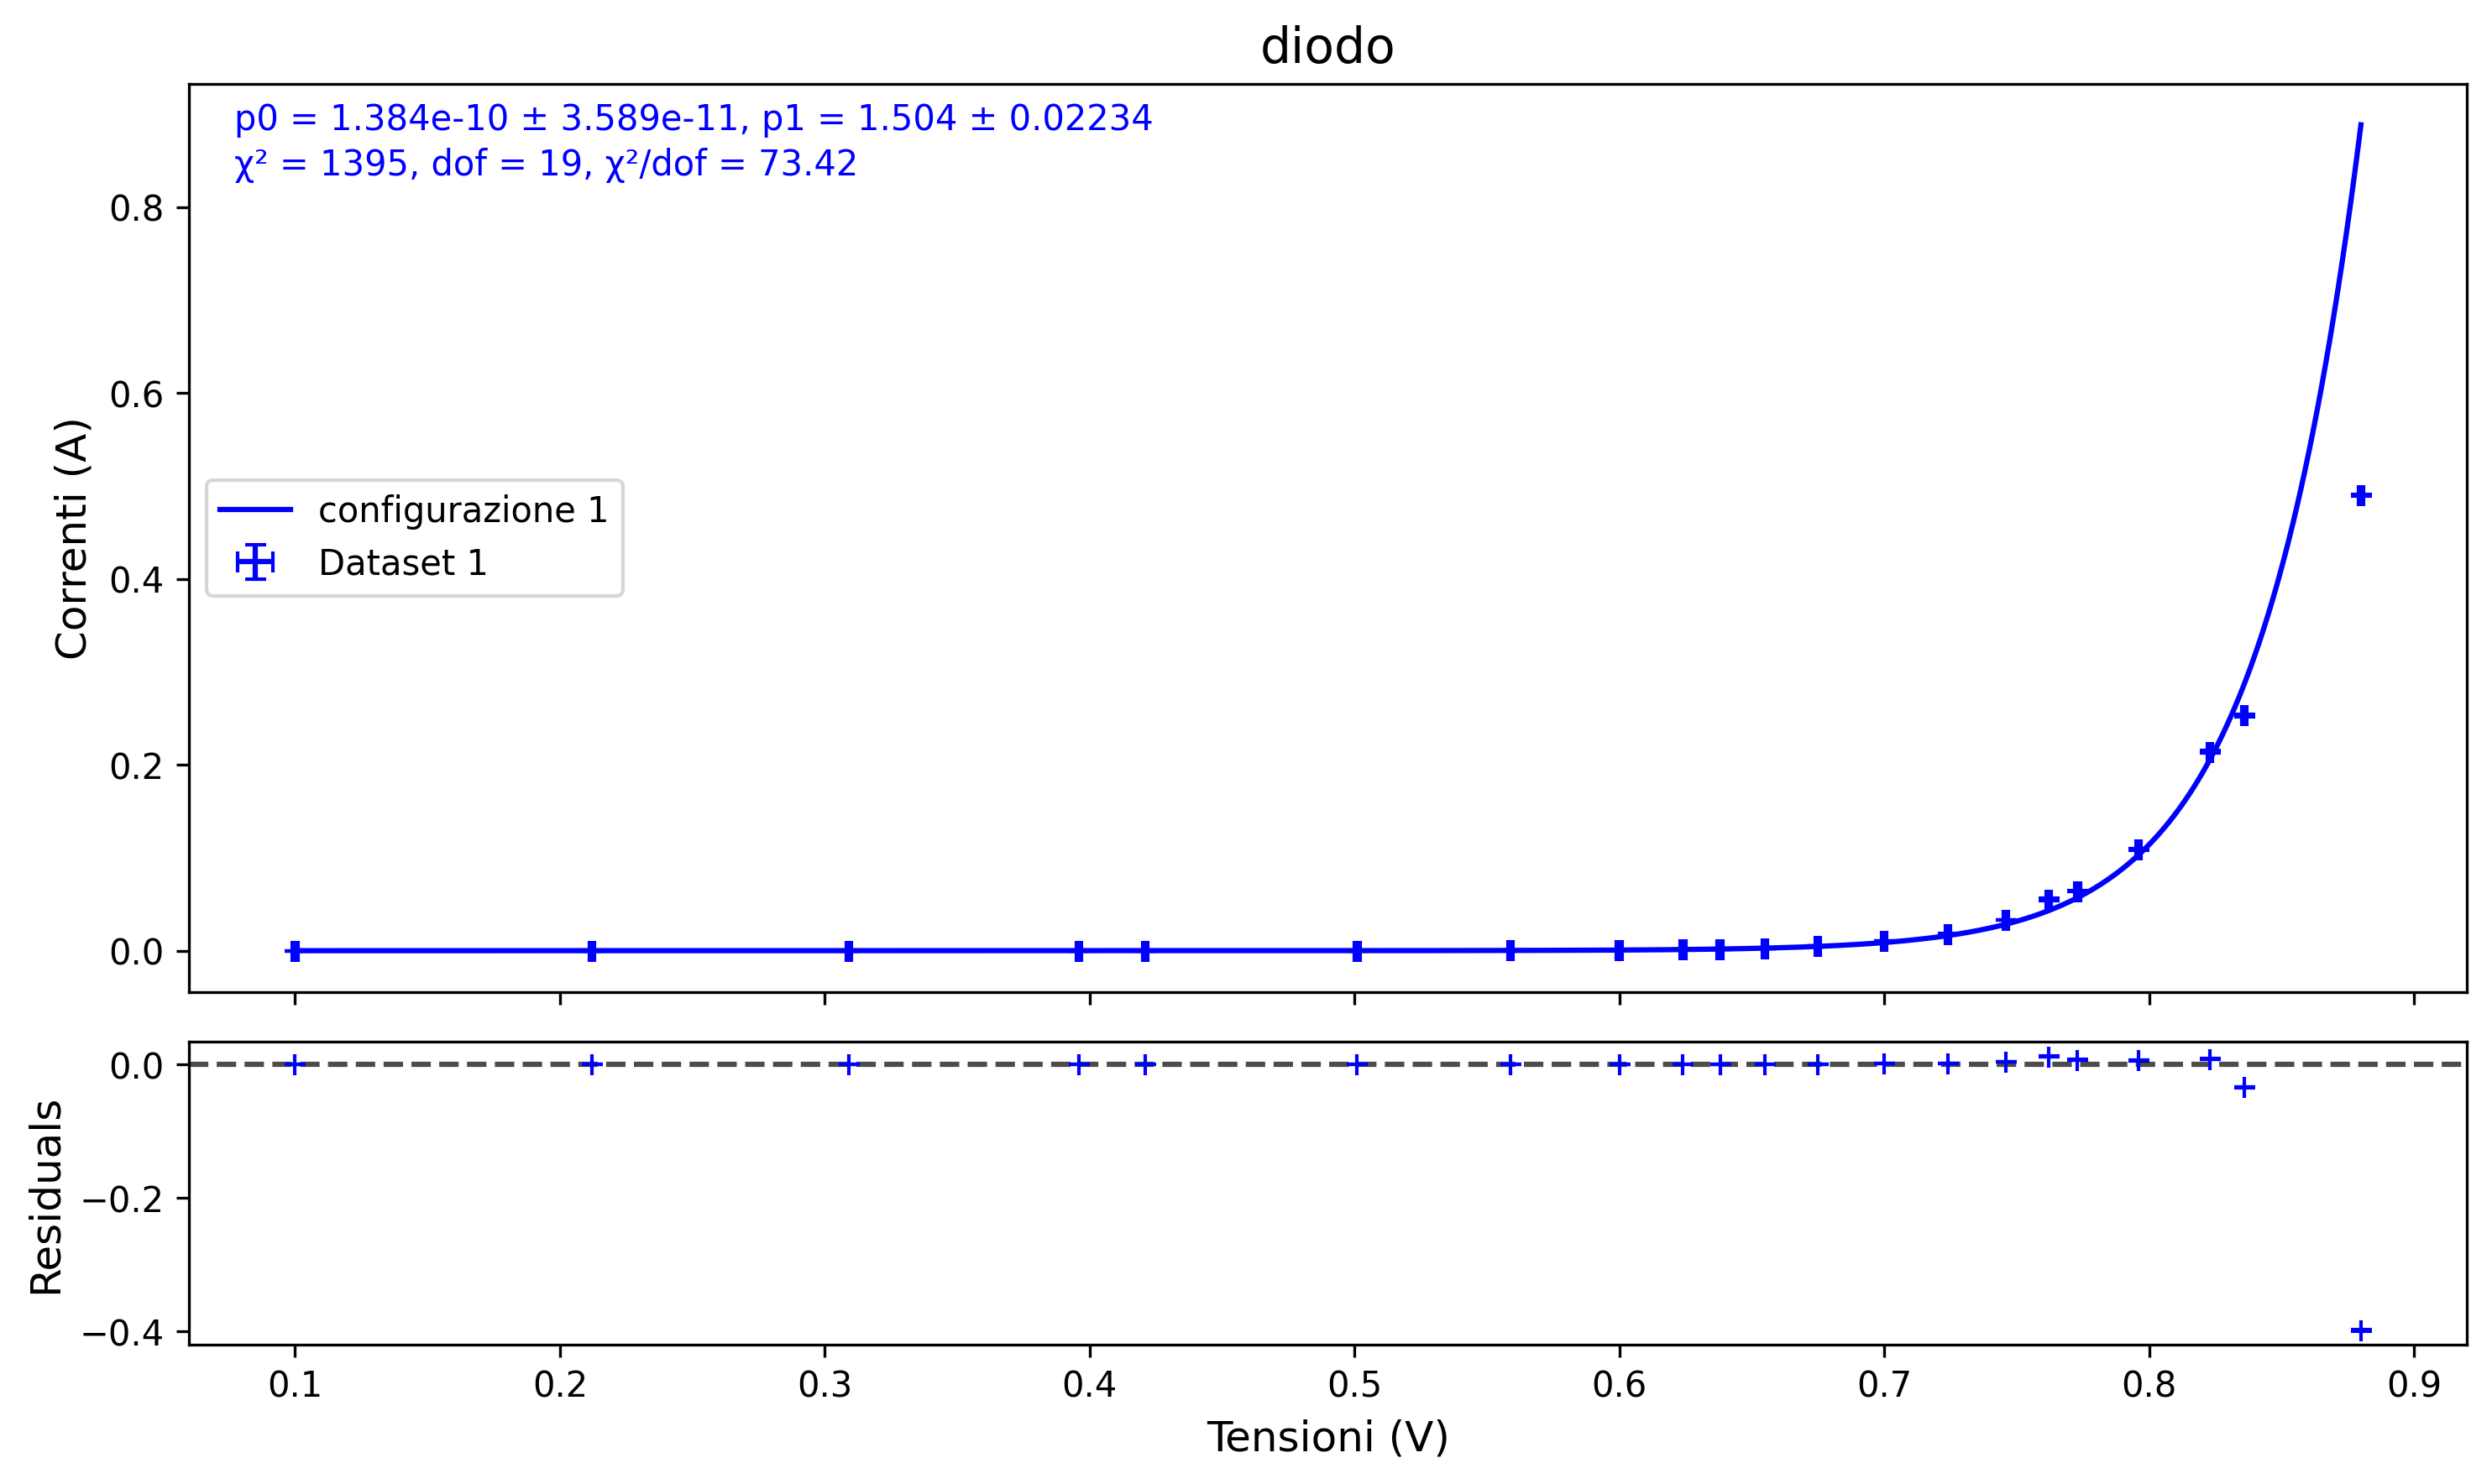
\includegraphics[width=0.75\linewidth]{grafici/diodo_1.png}
    \captionof{figure}{Diodo, configurazione 1}
    \label{fig:diodo 1}
\end{center}
\begin{center}
    \centering
    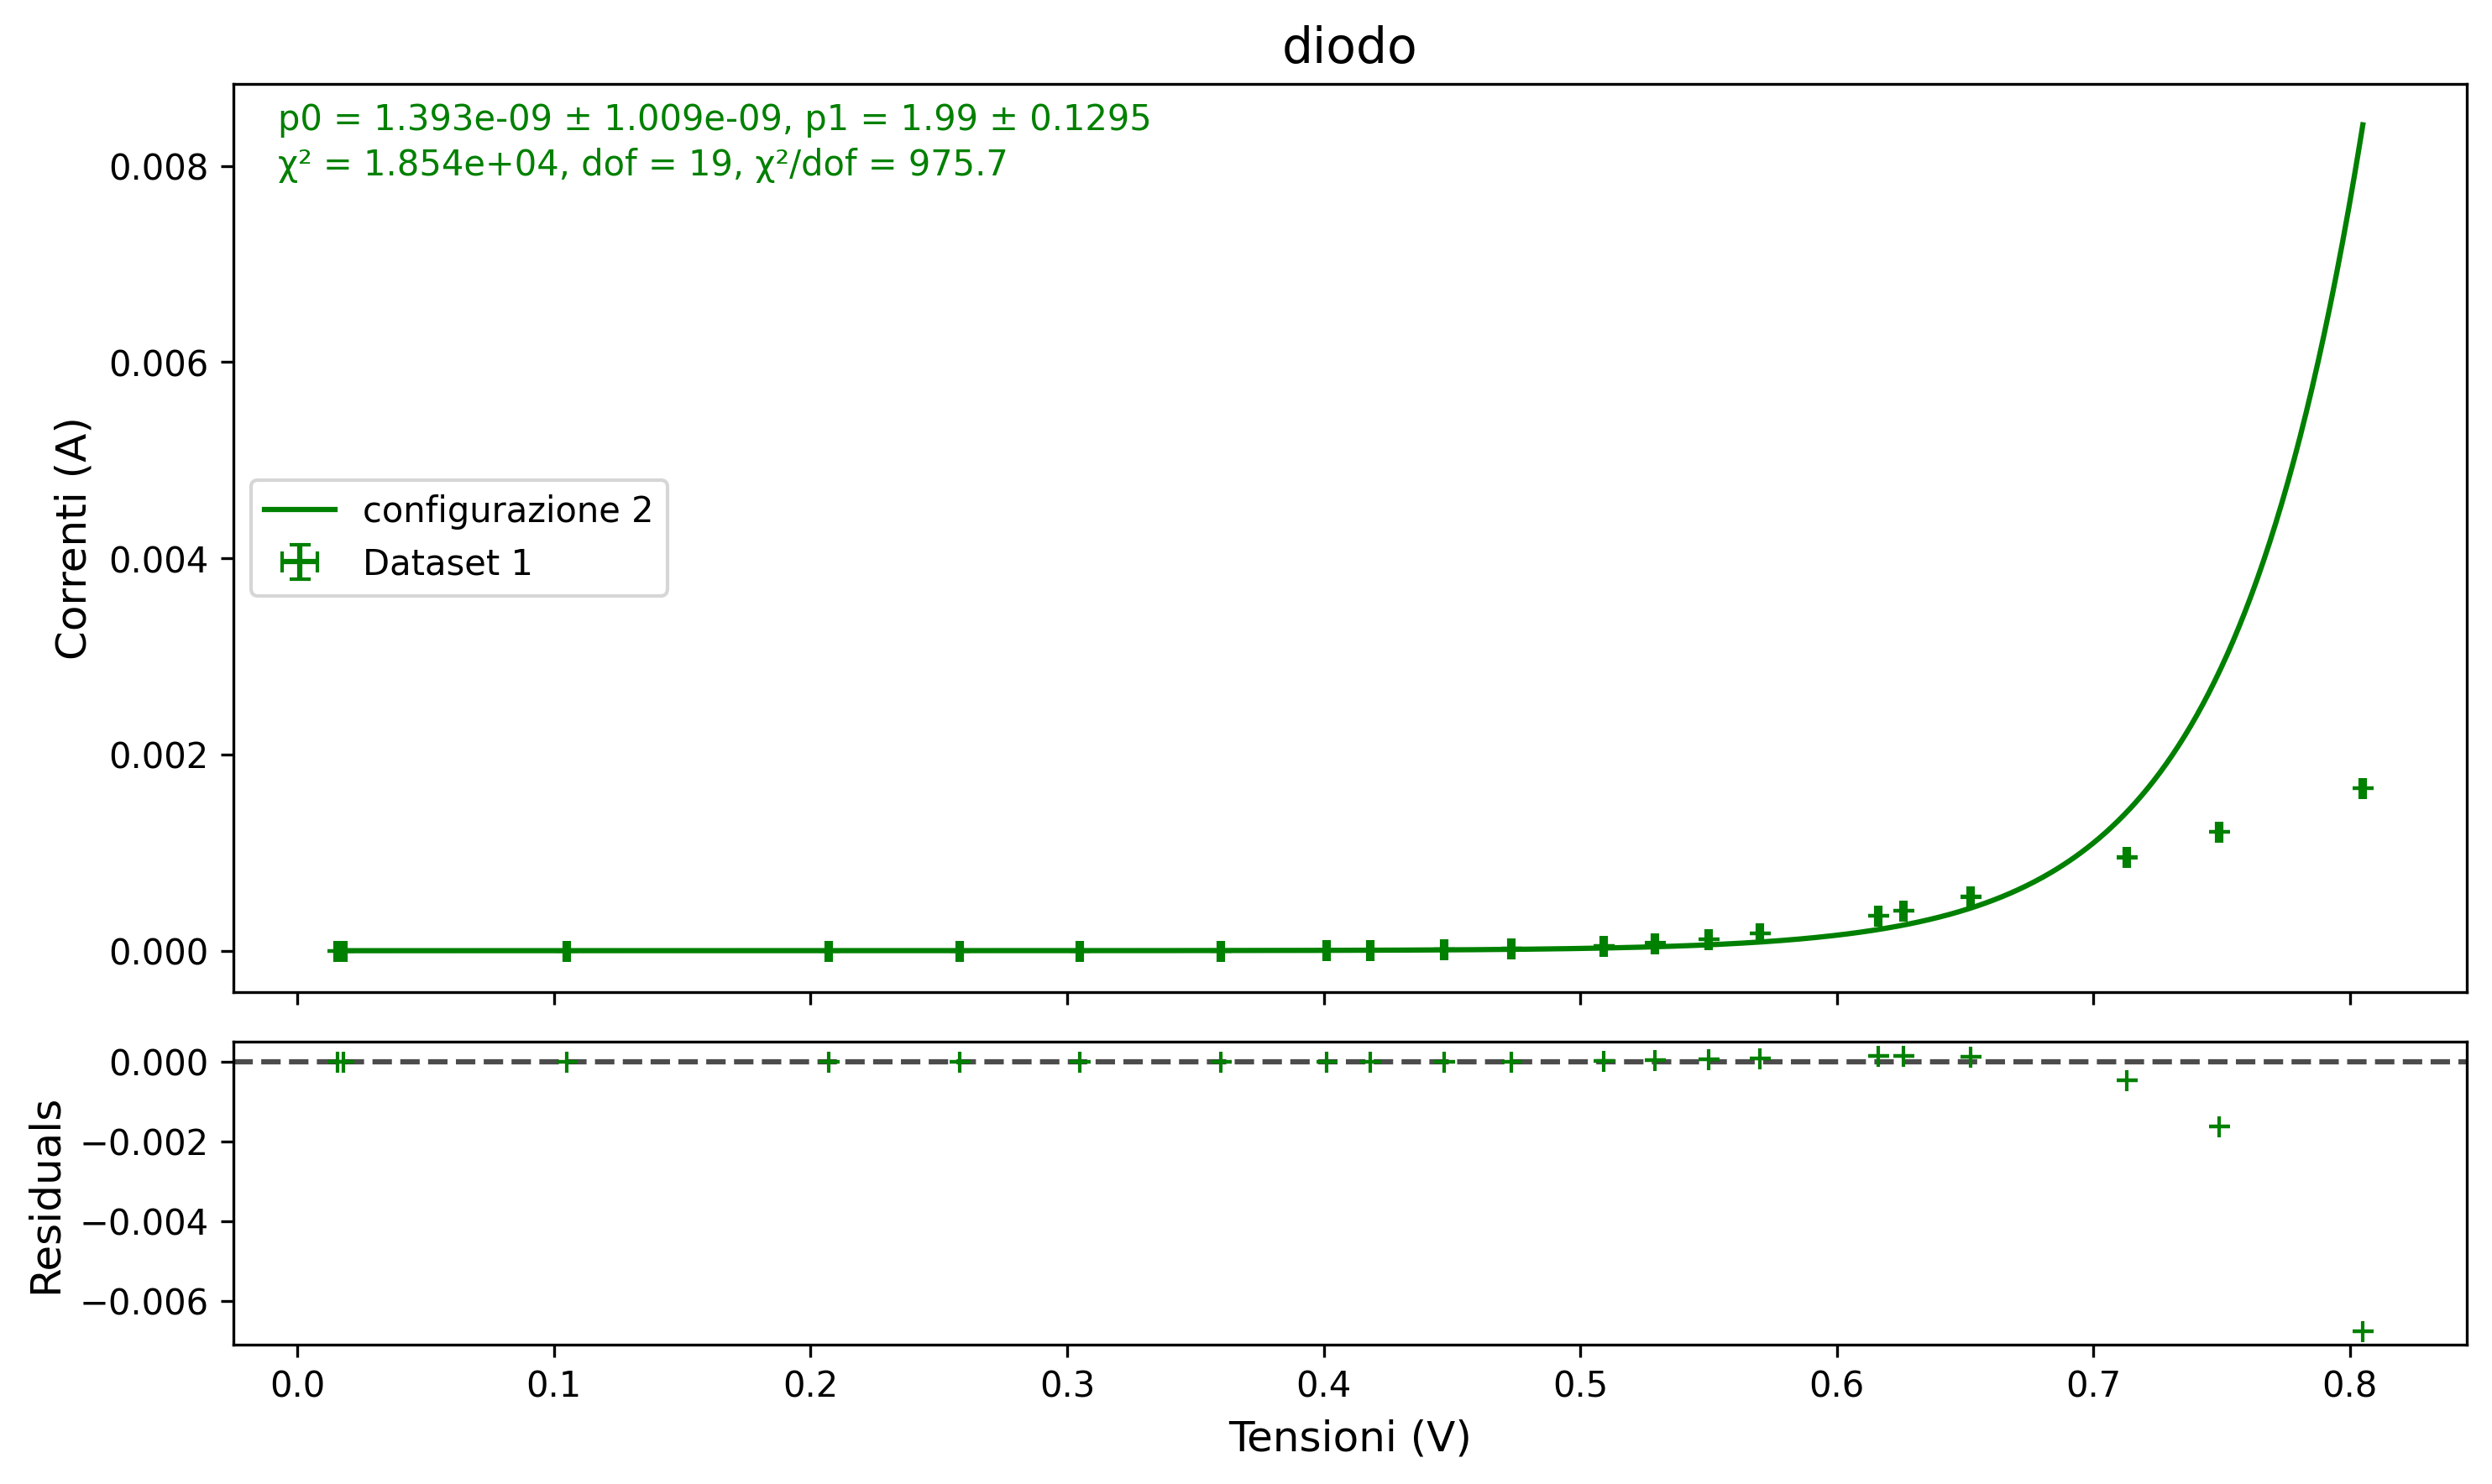
\includegraphics[width=0.75\linewidth]{grafici/diodo_2.png}
    \captionof{figure}{Diodo, configurazione 2}
    \label{fig:diodo 2}
\end{center}
Come si può notare dai risultati del test del chi quadro, per entrambe le configurazione il fit esponenziale non risulta essere un buon fit.
Per quanto riguarda la configurazione 2 ciò è giustificabile considerando che,          all'aumentare della tensione, la resistenza equivalente diminuisce esponenzialmente, e per resistenze basse abbiamo già illustrato come la configurazione 2 non garantisca buone misurazioni. 
Inoltre utilizzando la configurazione 2 siamo riusciti a raggiungere valori di corrente notevolmente più bassi rispetto a quelli misurati con la configurazione 1. Tale discrepanza è da attribuirsi alla non idealità degli strumenti di misura. Inserendo infatti il voltmetro a capi della serie amperometro-diodo la resistenza interna dell'amperometro ($R_a=1.8 \si{\ohm}$) "oscura" la resistenza del diodo $R_{\text{eq}}$, la quale per valori alti di corrente-tensione risulta dell'ordine di $\times 10^{-4}\si{\ohm}$. Di conseguenza non si riesce a misurare correttamente l'effetto del diodo sul circuito.
Tuttavia ciò non spiega il perchè anche la configurazione 1 fallisca quando si ha a che fare con tensioni alte e quindi resistenze equivalenti basse.
Una spiegazione di tale fenomeno si può imputare al fatto che la legge di Shokley dipenda esponenzialmente dall'inverso della temperatura del diodo, la quale aumenta con l'aumentare della corrente che attraversa il sistema. Dunque l'ipotesi che la temperatura sia costante durante tutto l'esperimento è errata, e la curva esponenziale ottenuta non è infine uguale a quella attesa. Sempre per la prima configurazione abbiamo tentato di interpolare solo i dati corrispondenti a resistenze equivalenti basse, cioè ad alte tensioni, e ad aumentare gli errori sulle correnti a un errore relativo del 10\%; infatti, nonostante questi non fossero considerati come la sensibilità dell'amperometro, ma come le fluttuazioni di misura, erano sottostimati: non tenevano conto delle incertezze dovute alla non idealità degli strumenti e alla temperatura non costante.

\begin{center}
    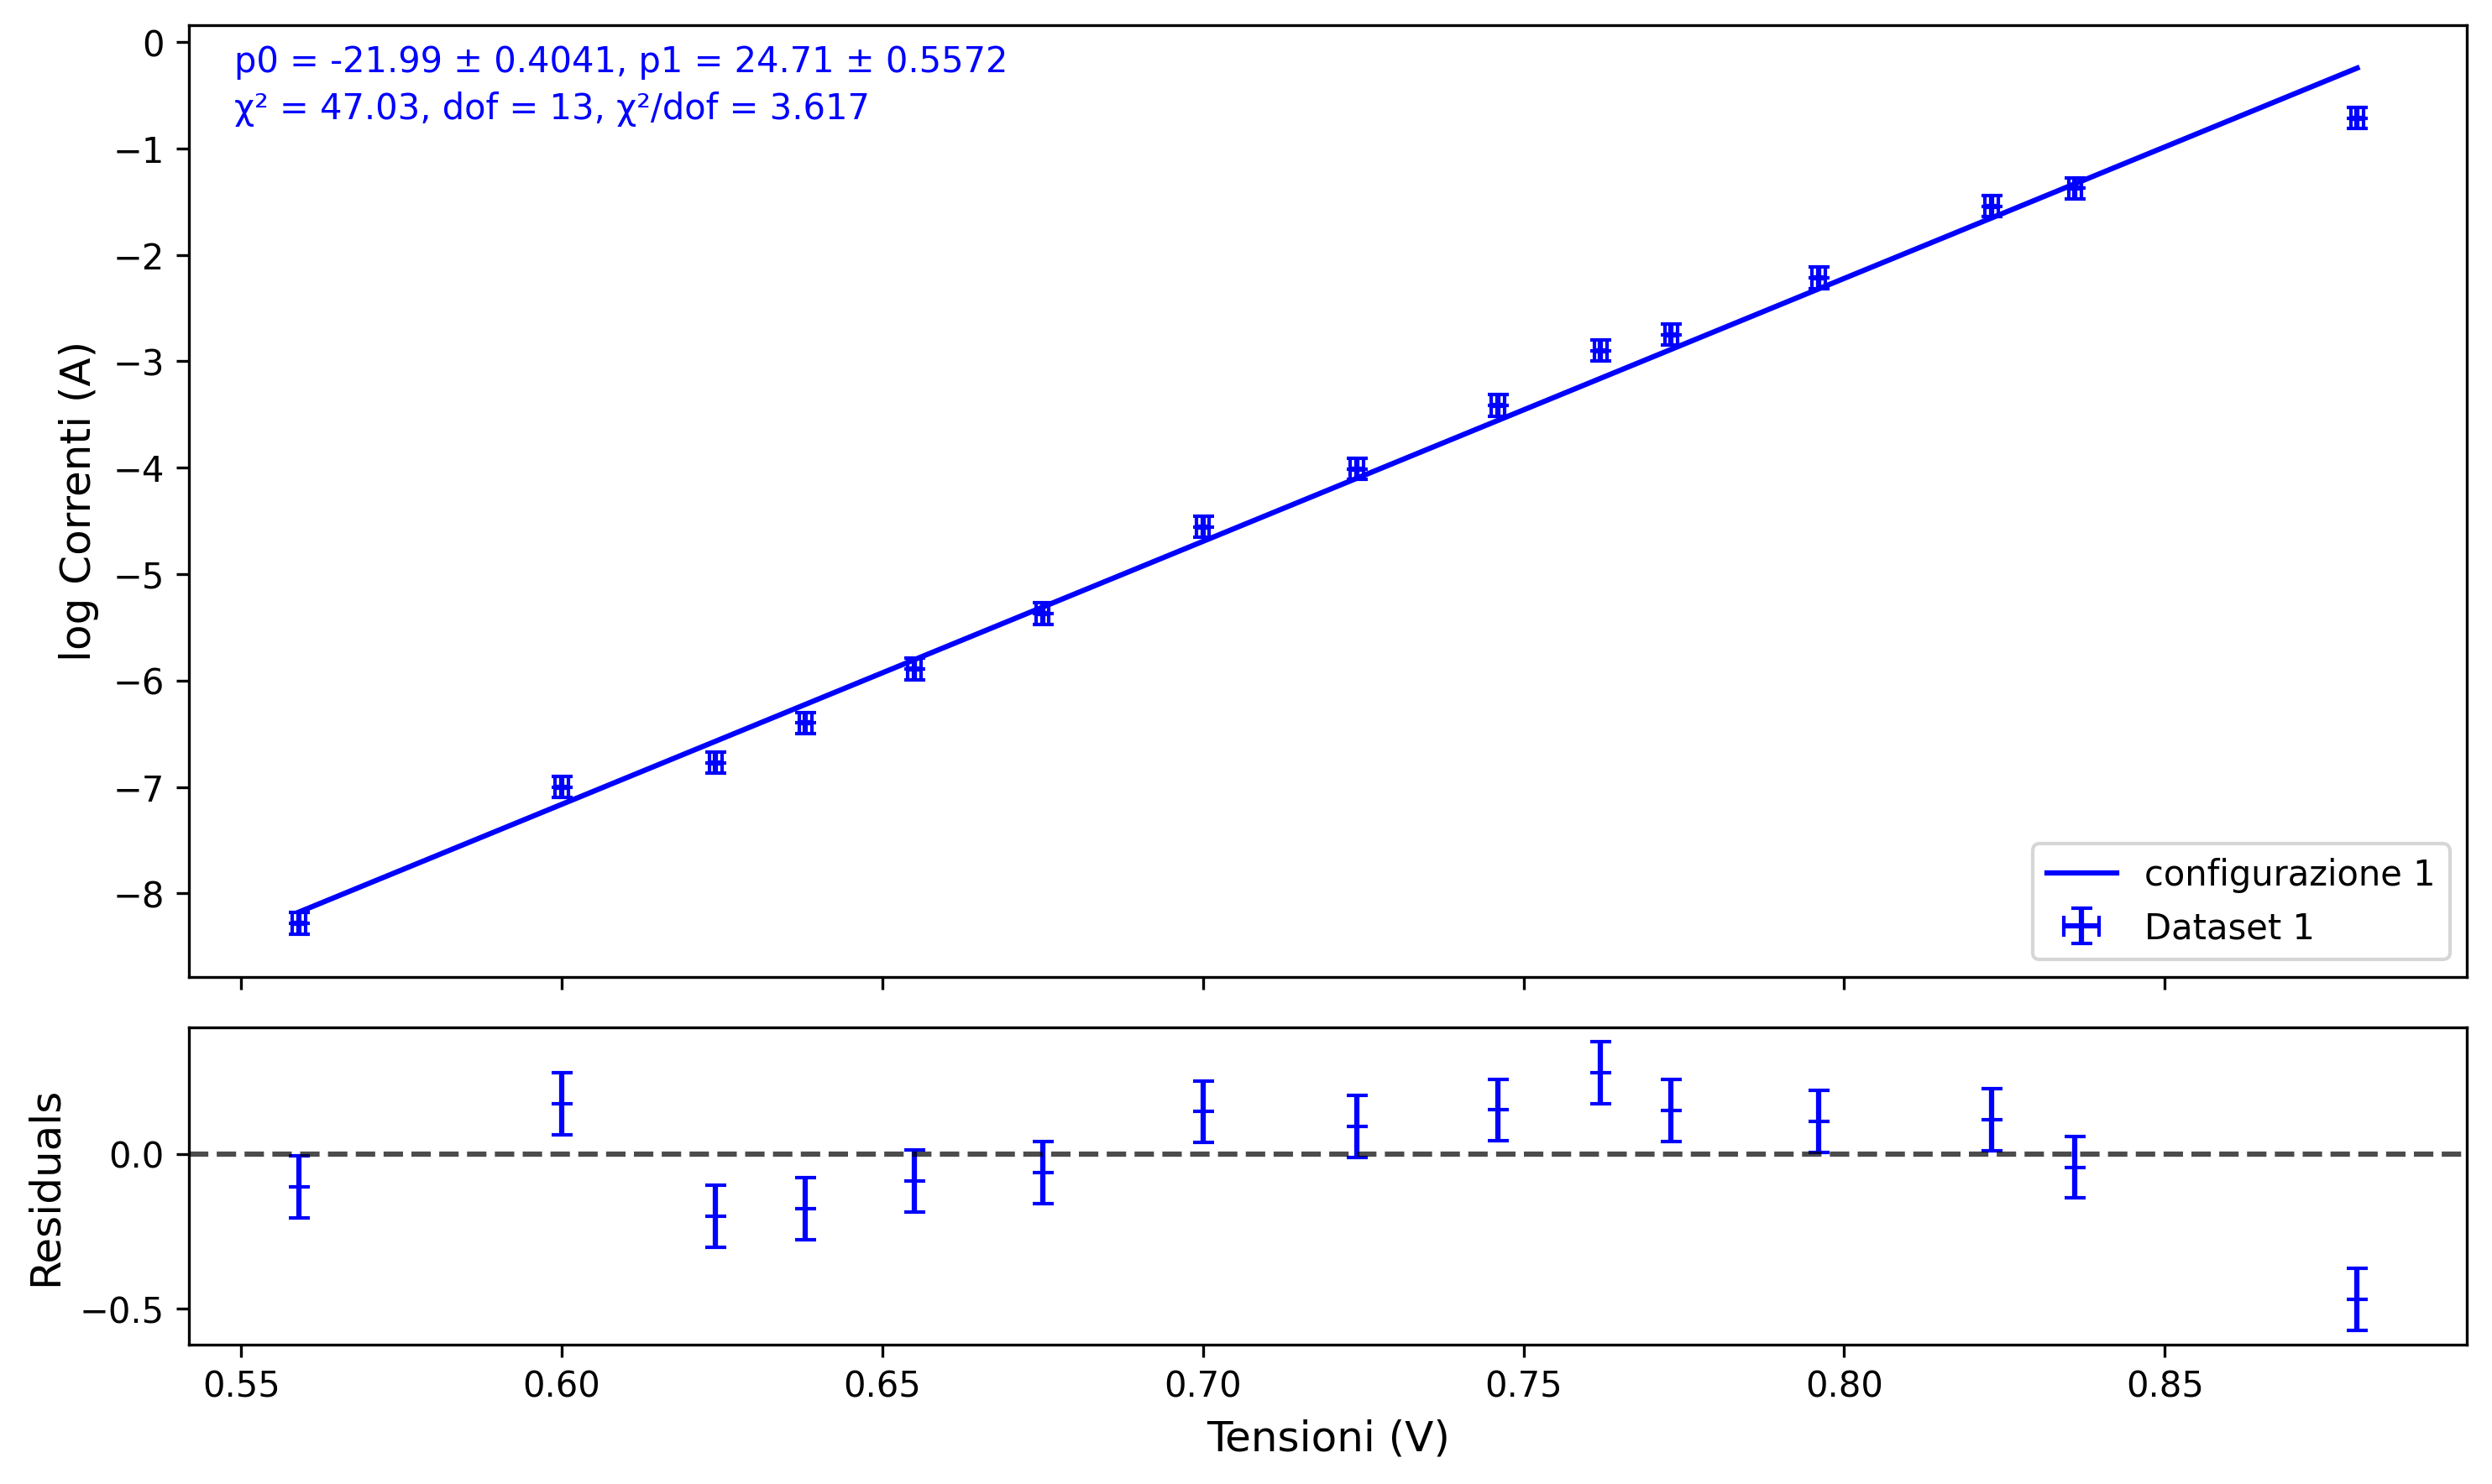
\includegraphics[width=0.7\textwidth]{grafici/diodo_sad.png}
    \captionof{figure}{Configurazione 1 con errore relativo del 10\%}
\end{center}
Dai parametri ottenuti risulta un chi quadro ridotto non compatibile con le misure \footnote{il chi quadro ridotto atteso è di 1 con deviazione standard stimata di $\sqrt{\frac{2}{13}} \approx 0.4$, e quello ottenuto dista circa 6 deviazioni standard}, certamente aumentando ancora gli errori si otterrebbe un risultato compatibile, tuttavia un errore relativo maggiore del 10\% non verificherebbe in modo attendibile la legge di Shockley.
\subsection{Conclusione}
In conclusione non possiamo dire verificata la legge di Shockley, dal momento che un fit esponenziale dei dati non è da considerarsi una buona interpolazione, come mostrato dai risultati del test del chi quadro, visibili nei grafici. Si può osservare inoltre che la curva interpolata cresce molto più rapidamente rispetto ai punti presi sperimentalmente. Ciò è concorde con l'aumento di temperatura dovuto a correnti alte; infatti il termine $T$, trovandosi al denominatore, al suo aumentare fa in modo che la curva si appiattisca. 
Riportiamo comunque una stima del valore della corrente di saturazione inversa $I_0$ e della costante $g$ propria del diodo. 
\begin{center}
\begin{tabular}{|c|c|}
\hline
$I_0[A]$ & $g$ \\
\hline
$(1.39 \pm 0.36)\times10^-10 $ & $1.50 \pm 0.02$ \\
\hline
\end{tabular}
\captionof{table}{parametri Legge di Shockley configurazione 1}
\end{center}
\begin{center}
\begin{tabular}{|c|c|}
\hline
$I_0 [A]$ & $g$ \\
\hline
$(1.39 \pm 1.01)\times10^-9 $ & $1.99 \pm 0.13$ \\
\hline
\end{tabular}
\captionof{table}{parametri Legge di Shockley configurazione 2}
\end{center}

%%%%%%%%%%%%%%%%%%%%%%%%%%%%%%%%%%%%%%%%%%%%%%%%%%%%%%%%%%%%%%%%%%%%%%%%%%%%%%%%%%%%%%%%%%


\section{Campo magnetico indotto da corrente}
\subsection{Obiettivo}
Verificare che il passaggio di corrente in una bobina generi un campo magnetico al suo interno.
Sfruttare una bussola per attuare le misurazioni, osservando come la corrente in circolo nella bobina incida sull'orientamento di un ago magnetico posto al suo interno.
\subsection{Metodo}
Abbiamo disposto il cellulare con l’app bussola sul supporto in modo tale che la bussola si trovasse al centro della bobina e che la direzione nord-sud da essa indicata
fosse perpendicolare all'asse del solenoide. In questo modo il campo magnetico generato dal passaggio di corrente (diretto lungo l'asse della bobina) aveva direzione perpendicolare
al campo magnetico terrestre (diretto lungo la direzione nord-sud). Abbiamo poi collegato la bobina all’alimentatore in regime di corrente continua e ne abbiamo aumentato gradualmente il valore,
osservando una progressiva rotazione dell'ago magnetico. Così facendo abbiamo raccolto 25 coppie di valori corrente-angolo di rotazione.
I valori di corrente sono stati utilizzati per determinare l'intensità del campo magnetico interno al solenoide, ricavato a partire dalla relazione \( B_s = \frac {\mu_0NI}{L} \),
dove \(\mu_0\) rappresenta la permeabilità magnetica del vuoto, \( \mathit{I} \) la corrente,
mentre \( \mathit{N=21} \) e \( \mathit{L=0.05m} \) indicano rispettivamente il numero di spire e la lunghezza del solenoide.
A partire dalle rotazioni è invece stata calcolata la tangente di ogni angolo.
\subsection{Dati}
Nella tabella e nel grafico sottostanti sono riportati i valori di corrente $I$ e dell'angolo di rotazione $\theta$.
Per la misura di entrambi abbiamo considerato come errore la sensibilità degli strumenti:
$\delta_I=0.01A$ (sensibilità del generatore di corrente) e $\delta_\theta=\SI{1}{\degree}$ (sensibilità della bussola).

\begin{center}
\begin{tabular}{|c|c|}
\hline
$\theta$ [°] & $I$ [A] \\
\hline
$0 \pm 1$ & $0.00 \pm 0.01$ \\
$3 \pm 1$ & $0.01 \pm 0.01$ \\
$8 \pm 1$ & $0.02 \pm 0.01$ \\
$13 \pm 1$ & $0.03 \pm 0.01$ \\
$15 \pm 1$ & $0.04 \pm 0.01$ \\
$20 \pm 1$ & $0.05 \pm 0.01$ \\
$24 \pm 1$ & $0.06 \pm 0.01$ \\
$27 \pm 1$ & $0.07 \pm 0.01$ \\
$30 \pm 1$ & $0.08 \pm 0.01$ \\
$36 \pm 1$ & $0.09 \pm 0.01$ \\
$38 \pm 1$ & $0.10 \pm 0.01$ \\
$40 \pm 1$ & $0.11 \pm 0.01$ \\
$43 \pm 1$ & $0.12 \pm 0.01$ \\
$47 \pm 1$ & $0.13 \pm 0.01$ \\
$48 \pm 1$ & $0.14 \pm 0.01$ \\
$50 \pm 1$ & $0.15 \pm 0.01$ \\
$53 \pm 1$ & $0.16 \pm 0.01$ \\
$55 \pm 1$ & $0.17 \pm 0.01$ \\
$58 \pm 1$ & $0.18 \pm 0.01$ \\
$60 \pm 1$ & $0.19 \pm 0.01$ \\
$61 \pm 1$ & $0.20 \pm 0.01$ \\
$63 \pm 1$ & $0.21 \pm 0.01$ \\
$64 \pm 1$ & $0.22 \pm 0.01$ \\
$66 \pm 1$ & $0.23 \pm 0.01$ \\
$67 \pm 1$ & $0.24 \pm 0.01$ \\
\hline
\end{tabular}
\captionof{table}{spostamento angolare indotto da corrente}
\end{center}

\begin{center}
    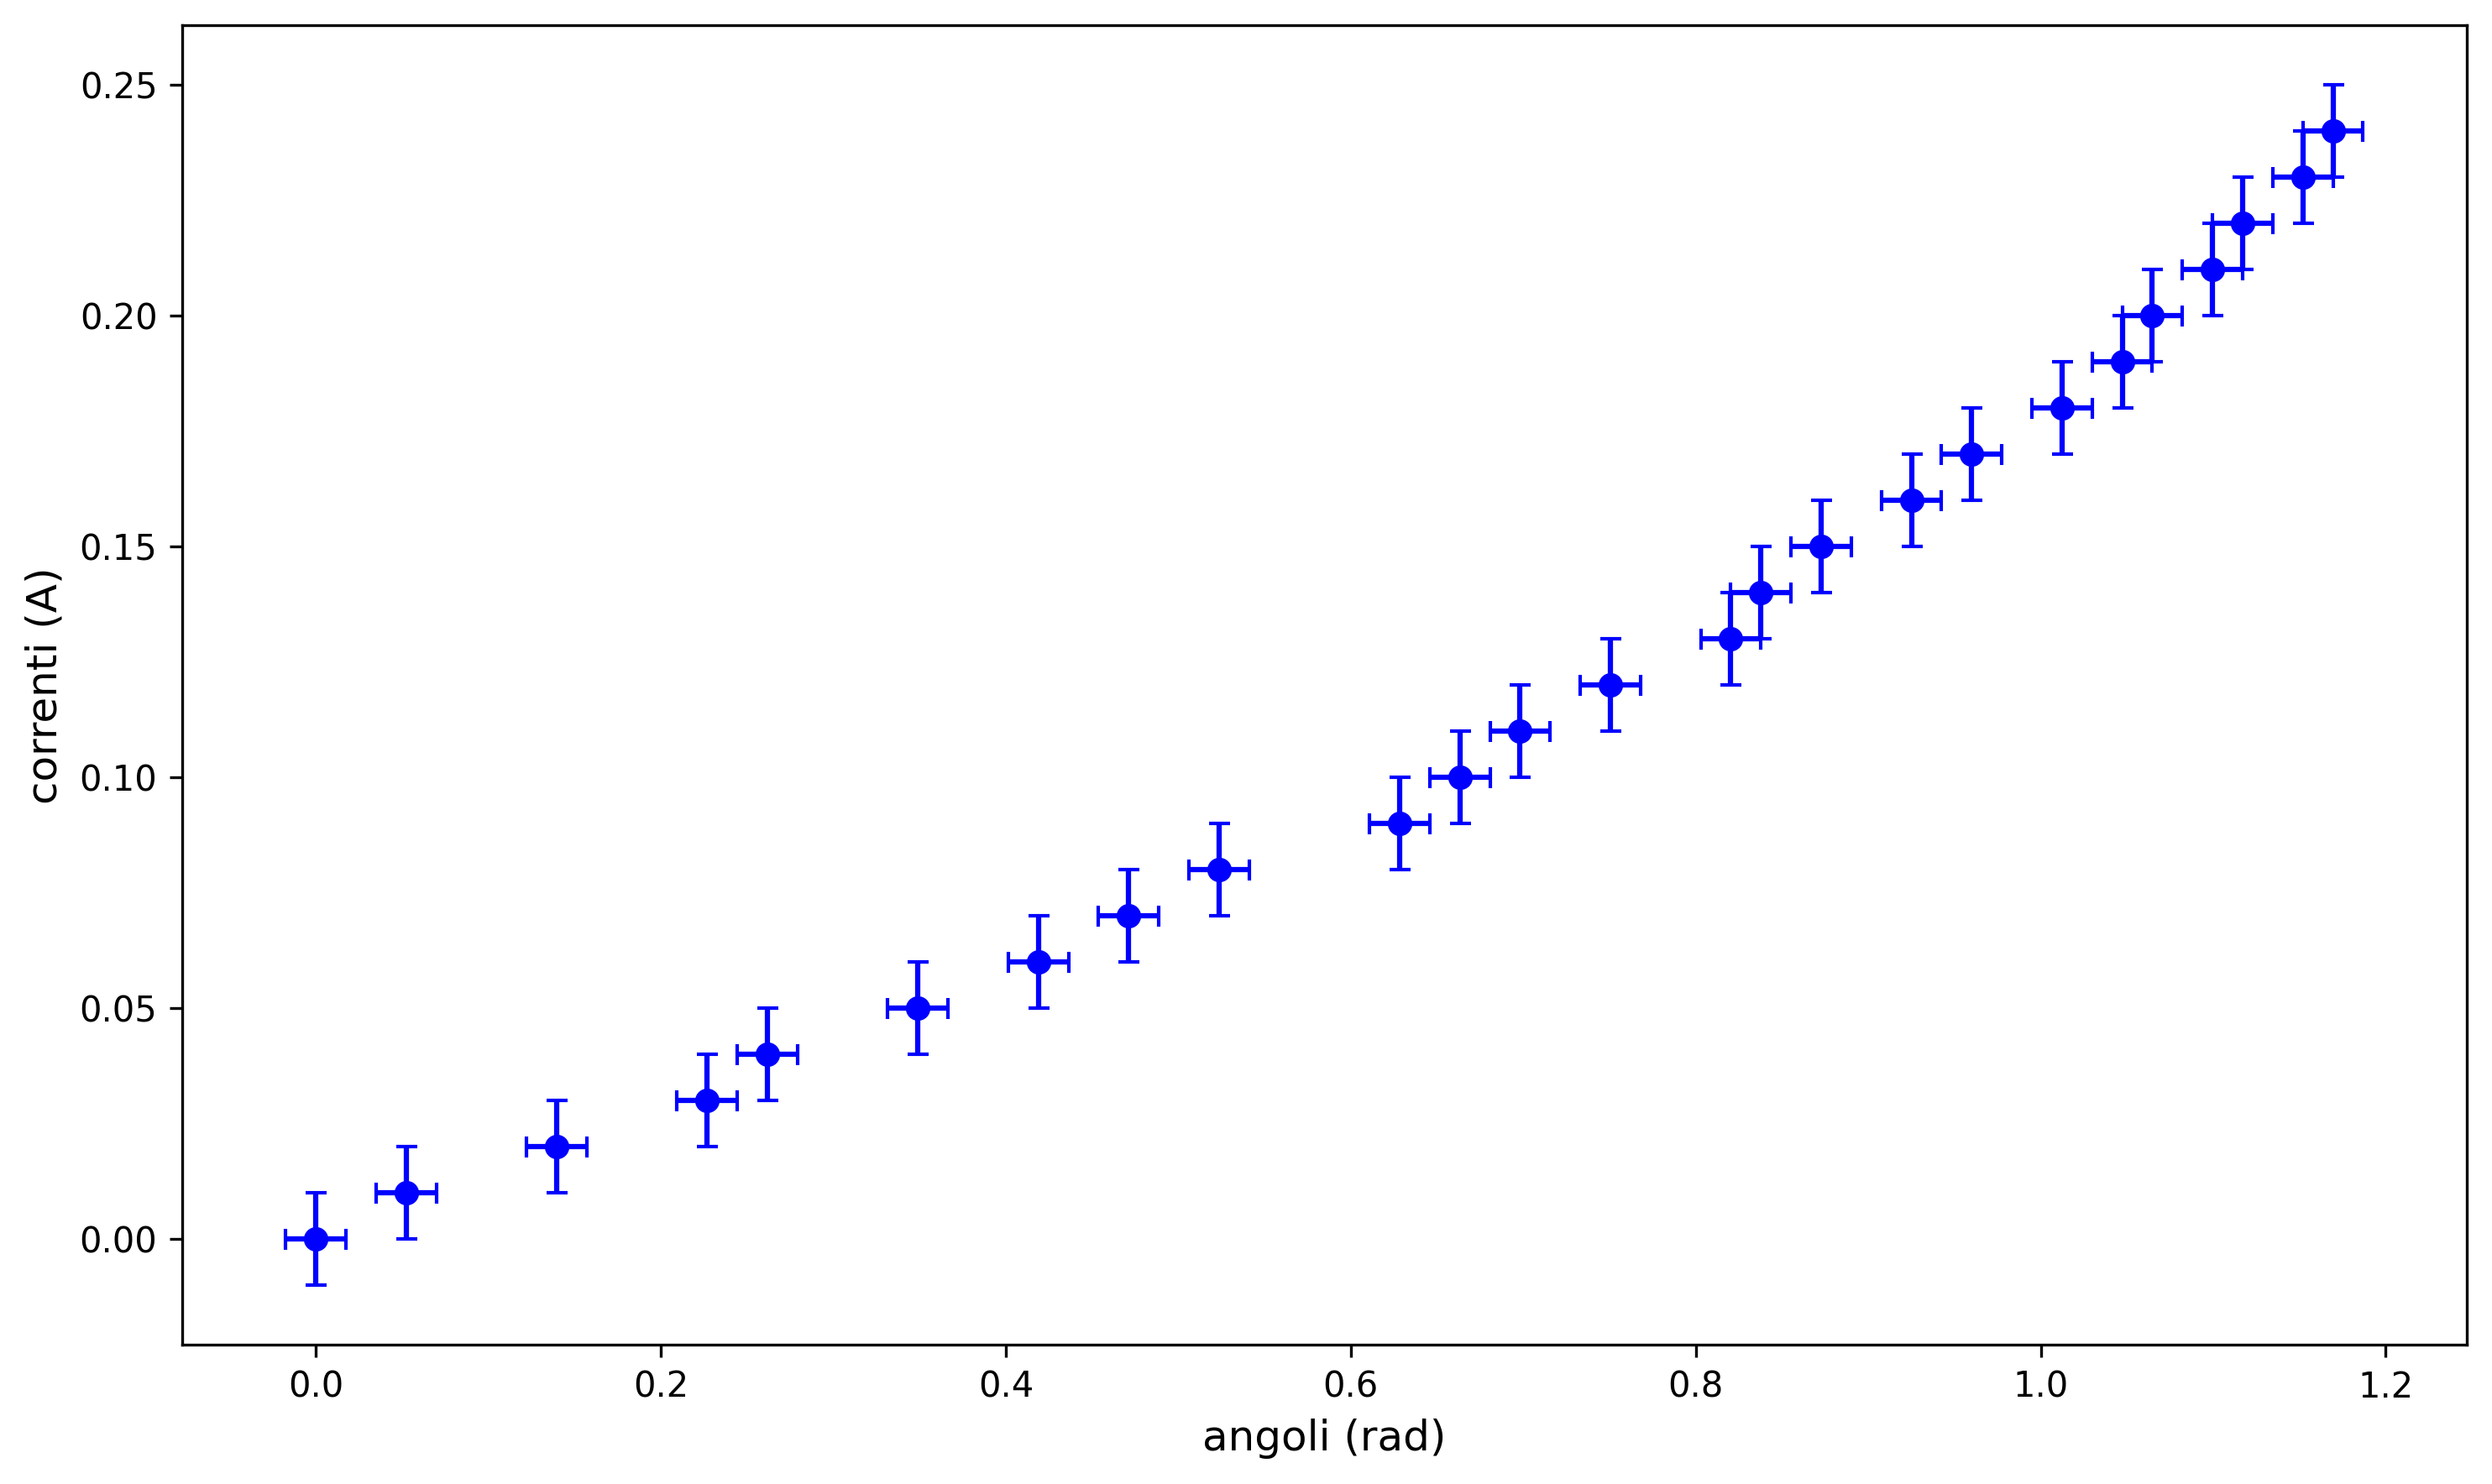
\includegraphics[width=0.8\textwidth]{grafici/bussola.png}
\end{center}
\subsection{Analisi dati}
Abbiamo riportato in figura i valori di $B_s$ e $\tan(\theta)$ con i rispettivi errori.
Per ricavare l'incertezza su $\tan(\theta)$ e $B_s$ sono state utilizzate le formule:
\begin{align*}
	 & \delta_{\tan} = \frac {1}{1+\theta^2}\delta_\theta \quad \text{e} \quad \delta_{B_s} = \frac {\mu_0N}{L}\delta_I
\end{align*}

\begin{center}
\begin{tabular}{|c|c|}
\hline
$B$ [T] & tan($\theta$) \\
\hline
$(0.0000 \pm 0.0078) \times 10^{-4}$ & $0.00 \pm 0.017$ \\
$(0.7791 \pm 0.0078) \times 10^{-5}$ & $0.05 \pm 0.017$ \\
$(1.5582 \pm 0.0078) \times 10^{-5}$ & $0.14 \pm 0.017$ \\
$(2.3373 \pm 0.0078) \times 10^{-5}$ & $0.23 \pm 0.0166$ \\
$(3.1165 \pm 0.0078) \times 10^{-5}$ & $0.27 \pm 0.0163$ \\
$(3.8956 \pm 0.0078) \times 10^{-5}$ & $0.36 \pm 0.0156$ \\
$(4.6747 \pm 0.0078) \times 10^{-5}$ & $0.45 \pm 0.0148$ \\
$(5.4538 \pm 0.0078) \times 10^{-5}$ & $0.51 \pm 0.0143$ \\
$(6.2329 \pm 0.0078) \times 10^{-5}$ & $0.58 \pm 0.0137$ \\
$(7.0120 \pm 0.0078) \times 10^{-5}$ & $0.73 \pm 0.0125$ \\
$(7.7911 \pm 0.0078) \times 10^{-5}$ & $0.78 \pm 0.0121$ \\
$(8.5703 \pm 0.0078) \times 10^{-5}$ & $0.84 \pm 0.0117$ \\
$(9.3494 \pm 0.0078) \times 10^{-5}$ & $0.93 \pm 0.0112$ \\
$(1.0128 \pm 0.0078) \times 10^{-4}$ & $1.07 \pm 0.0104$ \\
$(1.0908 \pm 0.0078) \times 10^{-4}$ & $1.11 \pm 0.0103$ \\
$(1.1687 \pm 0.0078) \times 10^{-4}$ & $1.19 \pm 0.0099$ \\
$(1.2466 \pm 0.0078) \times 10^{-4}$ & $1.33 \pm 0.0094$ \\
$(1.3245 \pm 0.0078) \times 10^{-4}$ & $1.43 \pm 0.0091$ \\
$(1.4024 \pm 0.0078) \times 10^{-4}$ & $1.60 \pm 0.0086$ \\
$(1.4803 \pm 0.0078) \times 10^{-4}$ & $1.73 \pm 0.0083$ \\
$(1.5582 \pm 0.0078) \times 10^{-4}$ & $1.80 \pm 0.0082$ \\
$(1.6361 \pm 0.0078) \times 10^{-4}$ & $1.96 \pm 0.0079$ \\
$(1.7141 \pm 0.0078) \times 10^{-4}$ & $2.05 \pm 0.0078$ \\
$(1.7919 \pm 0.0078) \times 10^{-4}$ & $2.25 \pm 0.0075$ \\
$(1.8699 \pm 0.0078) \times 10^{-4}$ & $2.36 \pm 0.0074$ \\
\hline
\end{tabular}
\end{center}

Tali dati sono stati poi interpolati con una legge di tipo lineare.
Ci aspettiamo infatti che essi siano legati dalla relazione $\tan(\theta) = \frac {B_s}{B_t}$ (dove $B_t$ indica il campo magnetico terrestre),
la quale esprime come la presenza di un campo magnetico esterno perpendicolare al campo terrestre causi uno spostamento angolare.

\begin{center}
    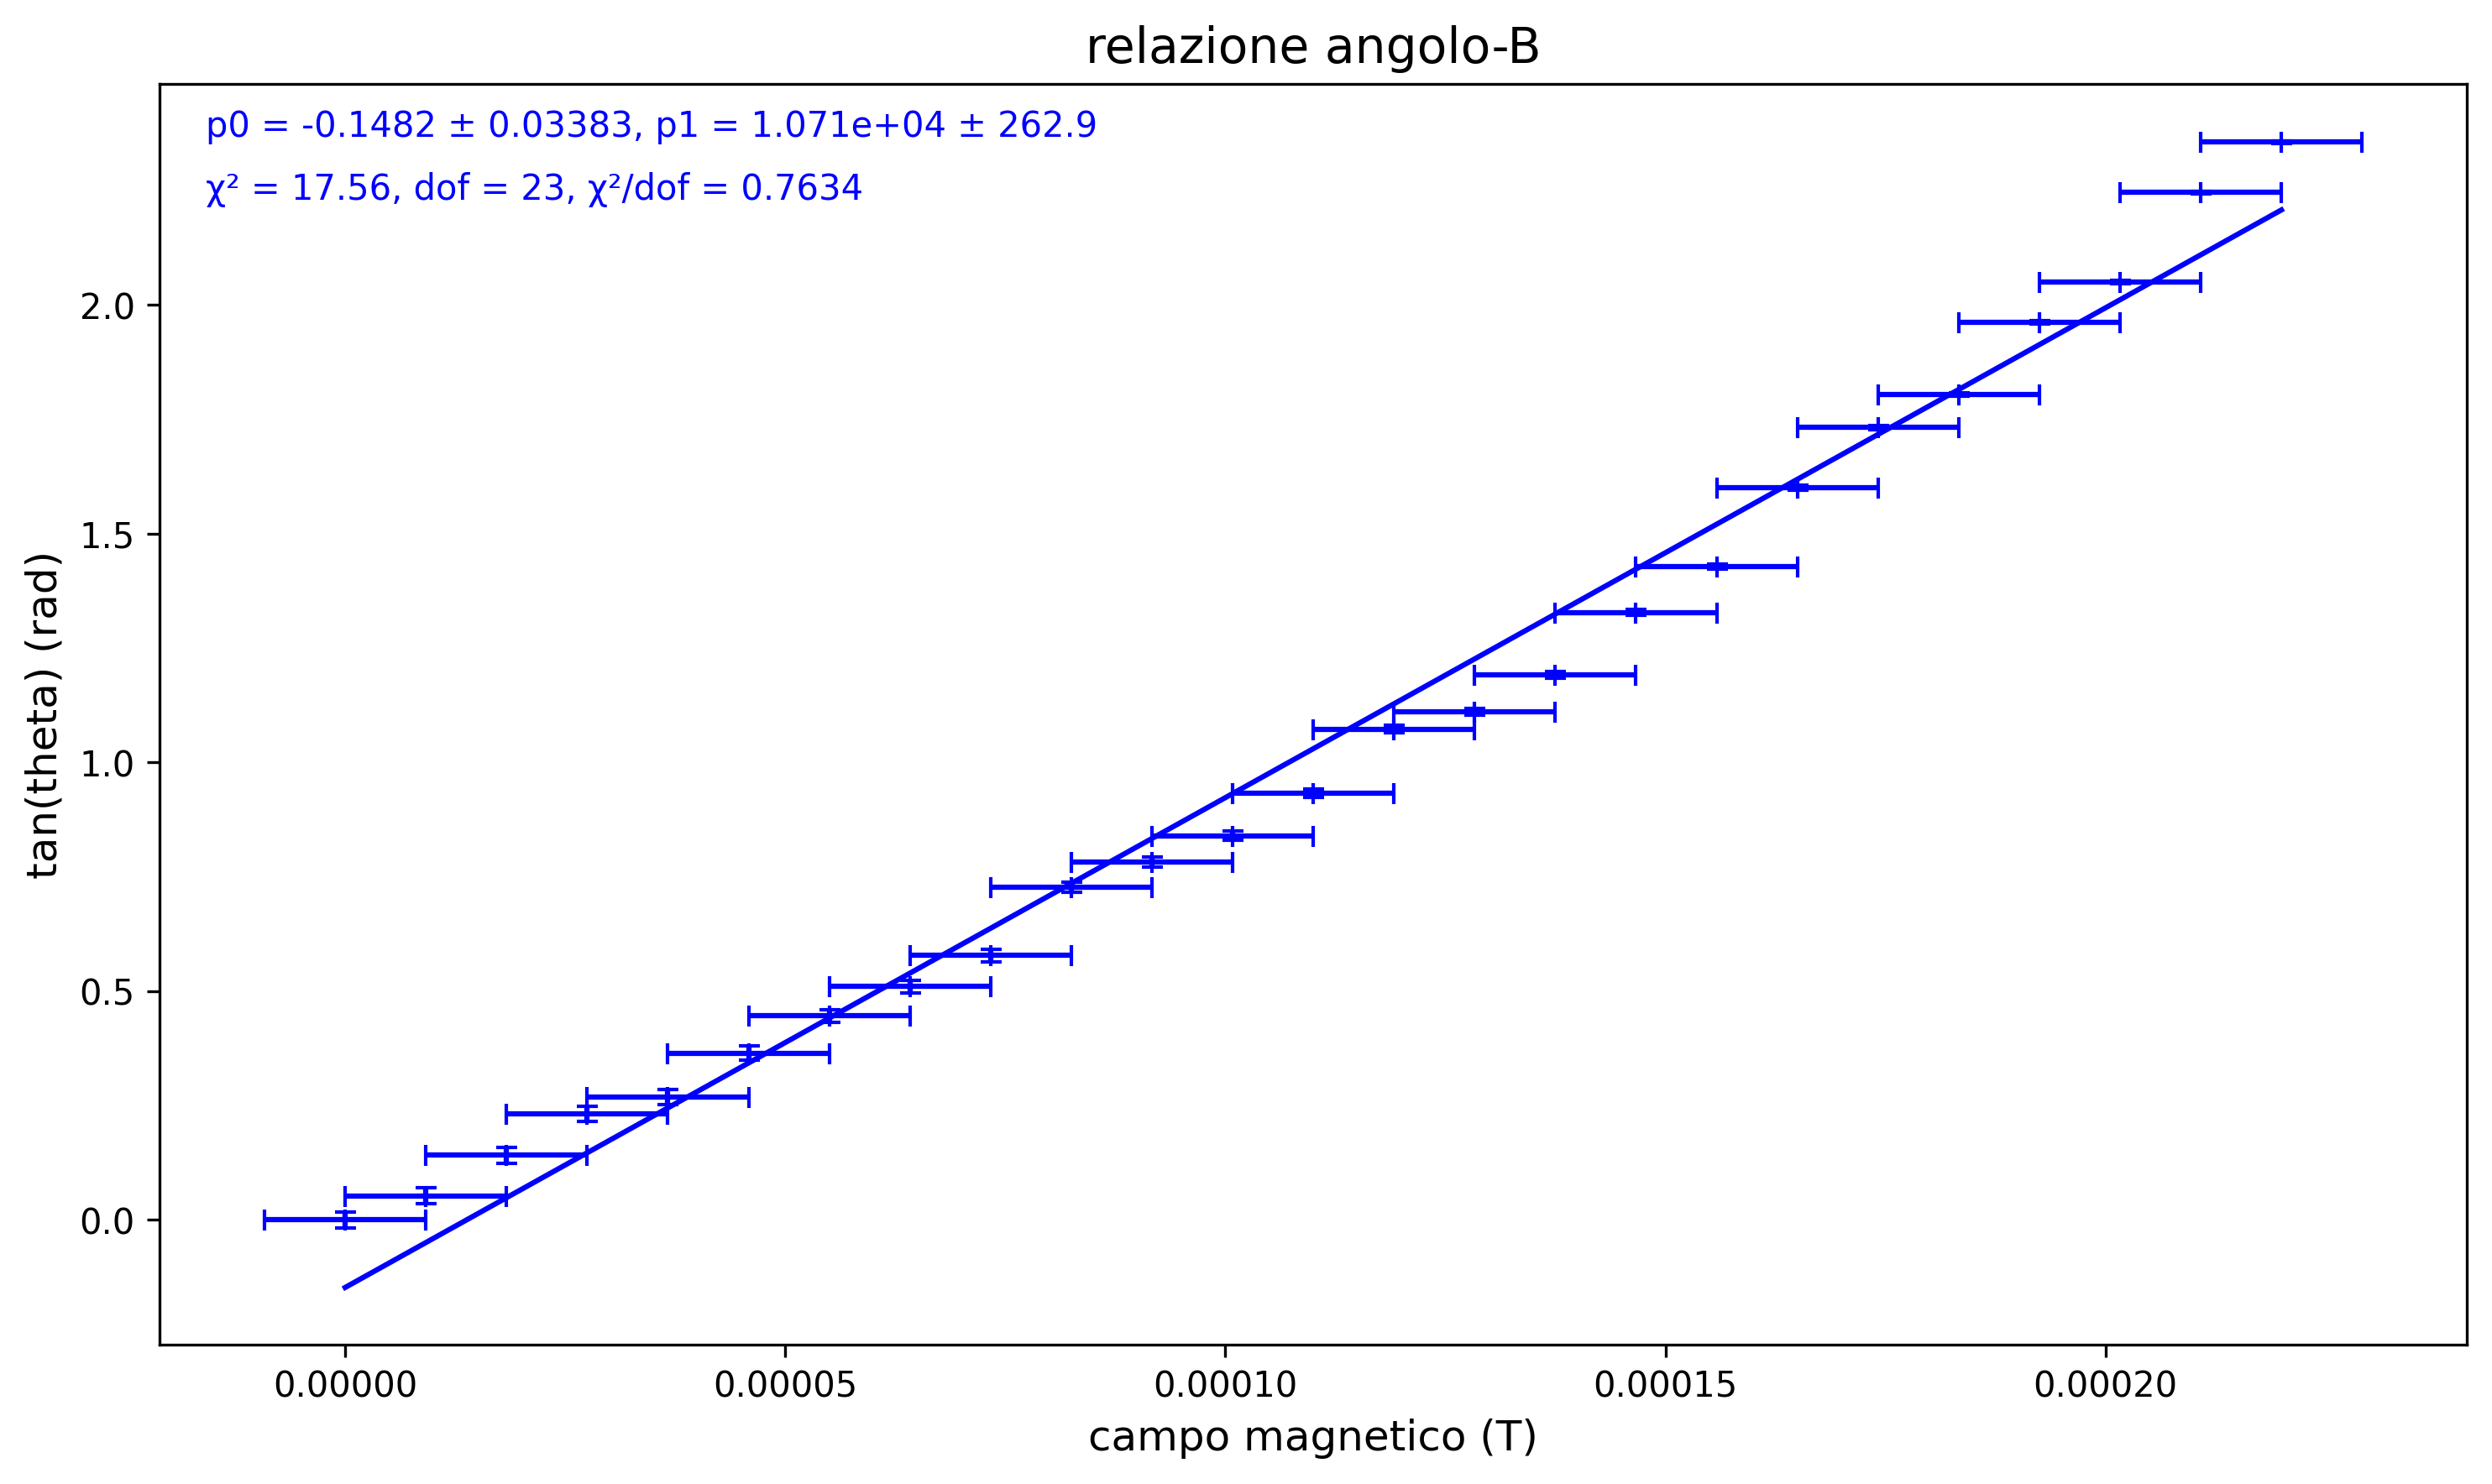
\includegraphics[width=0.8\textwidth]{grafici/campo_magnetico.png}
\end{center}
I risultati dell'interpolazione sono osservabili in seguito. $m$ indica il coefficiente angolare della retta e $a$ la sua intercetta,
$\delta_m$ e $\delta_a$ i loro errori.

\begin{center}
\begin{tabular}{|c|c|}
\hline
$m$ & $a$ \\
\hline
$10710.00 \pm 0.03$ & $-0.15 \pm 0.03$ \\
\hline
\end{tabular}
\captionof{table}{parametri retta}
\end{center}

\subsection{Conclusione}
A partire dai parametri ricavati tramite l'interpolazione lineare abbiamo potuto determinare una stima del campo magnetico terrestre;
possiamo infatti dedurre il campo magnetico terrestre dal coefficiente angolare della retta che meglio approssima la relazione tra i dati.
Risulta $B_t = \frac {1}{m}$ con errore $\delta_{B_t} = \frac {1}{m^2}\delta_m$.
I valori ottenuti sono raccolti nella tabella sottostante.

\begin{center}
\begin{tabular}{|l|c|}
\hline
$B_t$ [T] & $(7.9 \pm 0.2) \times 10^{-5}$ \\
\hline
\end{tabular}
\end{center}
\end{document}